\newpage
\section{TÍCH CỦA MỘT SỐ VỚI MỘT VÉC-TƠ}
\subsection{LÝ THUYẾT CẦN NHỚ}
\subsubsection{Tích của một số với một véc-tơ và các tính chất}
	\begin{enumerate}[\iconMT]
		\item \indam{Định nghĩa:}
		\begin{boxdn}
			Cho số $k\neq 0$ và véc-tơ $\overrightarrow{a} \neq \overrightarrow{0}$. Tích của số $k$ với véc-tơ $\overrightarrow{a}$ là một véc-tơ, kí hiệu là $k\overrightarrow{a}$, được xác định như sau
			\begin{itemize}
				\item Cùng hướng với $\overrightarrow{a}$ nếu $k>0$, ngược hướng với $\overrightarrow{a}$ nếu $k<0$.
				\item Có độ dài bằng $\left|k\right|\cdot\left|\overrightarrow{a}\right|$.
			\end{itemize}
			Ta quy ước $0\overrightarrow{a}=\overrightarrow{0}$ và $k\overrightarrow{0}=\overrightarrow{0}$.	
		\end{boxdn}
		\item \indam{Các tính chất:}
		\begin{boxdn}
			Với hai véc-tơ $\overrightarrow{a}$ và $\overrightarrow{b}$ bất kì; với mọi số thực $h$ và $k$, ta có:
			\begin{multicols}{3}
				\begin{itemize}
					\item $k\left(\overrightarrow{a}+\overrightarrow{b}\right)=k\overrightarrow{a}+k\overrightarrow{b}$.
					\item $1\cdot\overrightarrow{a}=\overrightarrow{a}$.
					\item $\left(h+k\right)\overrightarrow{a}=h\overrightarrow{a}+k\overrightarrow{a}$.
					\item $\left(-1\right)\cdot\overrightarrow{a}=-\overrightarrow{a}$.
					\item $h\left(k\overrightarrow{a}\right)=\left(hk\right)\overrightarrow{a}$.
				\end{itemize}
			\end{multicols}
		\end{boxdn}
	\end{enumerate}
%=================
\subsubsection{Điều kiện để hai véc-tơ cùng phương}
\begin{enumerate}[\iconMT]
	\item \indam{Định nghĩa:}
	\begin{boxdn}
		Hai véc-tơ $\overrightarrow{a}$ và $\overrightarrow{b}$ $\left(\overrightarrow{b} \text{ khác } \overrightarrow{0}\right)$ cùng phương khi và chỉ khi có số $k$ sao cho $\overrightarrow{a}=k\overrightarrow{b}$.
	\end{boxdn}
	\item \indam{Nhận xét:}
	\begin{boxdn}
		\begin{enumerate}
			\item Ba điểm $A$, $B$, $C$ thẳng hàng khi và chỉ khi có số $k$ khác $0$ để $\overrightarrow{AB}=k\overrightarrow{AC}$.
			\item Nếu $I$ là trung điểm của đoạn thẳng $AB$ thì $\overrightarrow{MA}+\overrightarrow{MB}=2\overrightarrow{MI}$ với điểm $M$ bất kì.
			\item Nếu $G$ là trọng tâm của tam giác $ABC$ thì $\overrightarrow{MA}+\overrightarrow{MB}+\overrightarrow{MC}=3\overrightarrow{MG}$  với điểm $M$ bất kì.
		\end{enumerate}
	\end{boxdn}
\end{enumerate}
%-------------------------------------------------------------------------------------------
\subsection{PHÂN LOẠI VÀ PHƯƠNG PHÁP GIẢI TOÁN}
\begin{dang}{Xác định điểm thoả mãn đẳng thức véc-tơ}
	Dựa vào định nghĩa, véc-tơ $k\overrightarrow{a}$ luôn cùng hướng với $\overrightarrow{a}$ nếu $k>0$, ngược hướng với $\overrightarrow{a}$ nếu $k<0$ và có độ dài bằng $\left|k\right|\cdot\left|\overrightarrow{a}\right|$.
\end{dang}
\begin{vd}%[0H5N3-3]%[Dự án D - Đề cương 3 khối 10-11-12 NH25-26 - Nguyễn Tiến]
	Cho đoạn thẳng $AB=3$ cm. Xác định các điểm $M$, $N$ thoả mãn $\overrightarrow{AM}=\dfrac{1}{3}\overrightarrow{AB}$, $\overrightarrow{AN}=-\dfrac{1}{3}\overrightarrow{AB}$.
	\loigiai{
		\immini{
			\begin{itemize}
				\item Do $\overrightarrow{AM} = \dfrac{1}{3} \overrightarrow{AB}$ nên $\overrightarrow{AM}$ và $\overrightarrow{AB}$ cùng hướng,
				$AM = \dfrac{1}{3} AB$.\\
				Vậy điểm $M$ thuộc tia $AB$ thoả mãn
				$AM = \dfrac{1}{3} AB = 1$ cm.
				\item Do $\overrightarrow{AN} = -\dfrac{1}{3}\overrightarrow{AB}$ nên $\overrightarrow{AN}$ và $\overrightarrow{AB}$ ngược hướng, $AN = \dfrac{1}{3}AB$.\\
				Vậy điểm $N$ thuộc tia đối của tia $AB$ thoả mãn $AN = \dfrac{1}{3}AB = 1$ cm.
			\end{itemize}
		}{
			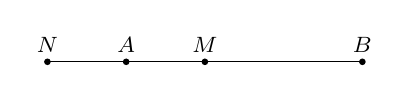
\begin{tikzpicture}[scale=1, font=\footnotesize, line join=round, line cap=round, >=stealth]
				\draw (-1,0)--(3,0);
				\foreach \x/\diem in {-1/N,0/A,1/M,3/B}
					\fill (\x,0) circle (1.2pt) node [above]{$\diem$};
			\end{tikzpicture}
		}
	}
\end{vd}
\begin{vd}%[0H5H3-3]%[Dự án D - Đề cương 3 khối 10-11-12 NH25-26 - Nguyễn Tiến]
	Cho tam giác $ABC$. Xác định điểm $M$ thoả mãn $\overrightarrow{AM} = 2\left(\overrightarrow{AB} + \overrightarrow{AC}\right)$.
	\loigiai{
		\immini{
			Dựng hình bình hành $ABDC$.\\
			Ta có $\overrightarrow{AD} = \overrightarrow{AB} + \overrightarrow{AC}$.\\
			Suy ra
			$$\overrightarrow{AM} = 2\left(\overrightarrow{AB} + \overrightarrow{AC}\right) \Leftrightarrow \overrightarrow{AM} = 2\overrightarrow{AD}.$$
			Vậy $M$ là điểm thuộc tia $AD$ thoả mãn $AM = 2AD$.
		}{
			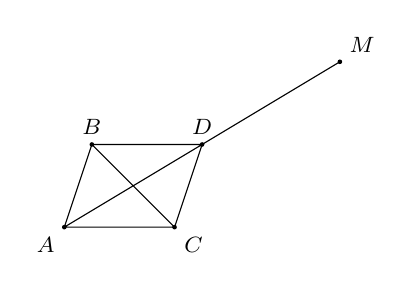
\begin{tikzpicture}[scale=0.7, font=\footnotesize, line join=round, line cap=round, >=stealth]
				\draw (0,0)node [below left]{$A$}--(2,0)node [below right]{$C$}--(2.5,1.5)node [above]{$D$}--(0.5,1.5)node [above]{$B$}--(0,0)--(5,3)node [above right]{$M$} (0.5,1.5)--(2,0);
				\foreach \x/\y in {0/0,2/0,2.5/1.5,0.5/1.5,5/3}
					\fill (\x,\y) circle (1.2pt);
			\end{tikzpicture}
		}
	}
\end{vd}
\begin{vd}%[0H5H3-3]%[Dự án D - Đề cương 3 khối 10-11-12 NH25-26 - Nguyễn Tiến]
	Cho tứ giác $ABCD$. Xác định điểm $M$ thoả mãn $3\overrightarrow{MA} + \overrightarrow{MB} + \overrightarrow{MC} + \overrightarrow{MD} = \overrightarrow{0}$.
	\loigiai{
		Gọi $G$ là trọng tâm của tam giác $BCD$, ta có $\overrightarrow{MB} + \overrightarrow{MC} + \overrightarrow{MD} = 3\overrightarrow{MG}$.\\
		Suy ra
		\allowdisplaybreaks
		\begin{eqnarray*}
			& & 3\overrightarrow{MA} + \overrightarrow{MB} + \overrightarrow{MC} + \overrightarrow{MD} = \overrightarrow{0}\\
			&\Leftrightarrow & 3\overrightarrow{MA} + 3\overrightarrow{MG} = \overrightarrow{0} \Leftrightarrow \overrightarrow{MA} + \overrightarrow{MG} = \overrightarrow{0}.
		\end{eqnarray*}
		Vậy $M$ là trung điểm của đoạn thẳng $AG$.
	}
\end{vd}
%=================
\begin{dang}{Biểu thị một véc-tơ theo một véc-tơ cùng phương}
	\textit{Phương pháp}: Sử dụng tính chất sau
	\begin{itemize}
		\item Nếu hai véc-tơ $\overrightarrow{a}$ và $\overrightarrow{b}$ $\left(\overrightarrow{b}\neq \overrightarrow{0}\right)$ cùng hướng và $\left|\overrightarrow{a}\right| = m\cdot\left|\overrightarrow{b}\right|$ thì $\overrightarrow{a} = m\overrightarrow{b}$.
		\item Nếu hai véc-tơ $\overrightarrow{a}$ và $\overrightarrow{b}$ $\left(\overrightarrow{b}\neq \overrightarrow{0}\right)$ ngược hướng và $\left|\overrightarrow{a}\right| = m\cdot\left|\overrightarrow{b}\right|$ thì $\overrightarrow{a} = -m\overrightarrow{b}$.
	\end{itemize}
\end{dang}
\begin{vd}%[0H5N3-1]%[Dự án D - Đề cương 3 khối 10-11-12 NH25-26 - Nguyễn Tiến]
	\immini{
		Cho tam giác $ABC$ có $G$ là trọng tâm và $M$ là trung điểm của $BC$.
		\begin{enumerate}
			\item Biểu thị $\overrightarrow{AG}$ theo $\overrightarrow{AM}$.
			\item Biểu thị $\overrightarrow{GA}$ theo $\overrightarrow{GM}$.
		\end{enumerate}
	}{
		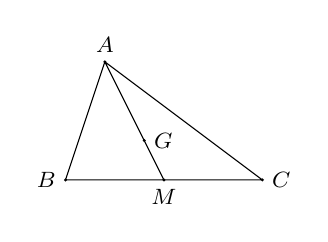
\begin{tikzpicture}[scale=0.5, font=\footnotesize, line join=round, line cap=round, >=stealth]
			\draw (1,3)node [above]{$A$}--(0,0)node [left]{$B$}--(5,0)node [right]{$C$}--(1,3)--(2,1)node [right]{$G$}--(2.5,0)node [below]{$M$};
			\foreach \x/\y in {0/0,1/3,5/0,2/1,2.5/0}
				\fill (\x,\y) circle (1.2pt);
		\end{tikzpicture}
	}
	\loigiai{
		\begin{enumerate}
			\item Vì $\overrightarrow{AG}$ và $\overrightarrow{AM}$ cùng hướng và $\left|\overrightarrow{AG}\right| = \dfrac{2}{3} \left|\overrightarrow{AM}\right|$ nên $\overrightarrow{AG} = \dfrac{2}{3}\overrightarrow{AM}$.
			\item Vì $\overrightarrow{GA}$ và $\overrightarrow{GM}$ ngược hướng và $\left|\overrightarrow{GA}\right| = 2\left|\overrightarrow{GM}\right|$ nên $\overrightarrow{GA} = -2\overrightarrow{GM}$.
		\end{enumerate}
	}
\end{vd}
%=================
\begin{dang}{Biểu thị một véc-tơ theo hai véc-tơ không cùng phương}
	\textit{Phương pháp}:
	\begin{itemize}
		\item Sử dụng định nghĩa, tính chất của các phép toán: phép cộng véc-tơ, phép trừ véc-tơ, phép nhân một số với một véc-tơ.
		\item Sử dụng tính chất trung điểm của đoạn thẳng, trọng tâm của tam giác, hình bình hành.
	\end{itemize}
\end{dang}
\begin{vd}%[0H5H3-5]%[Dự án D - Đề cương 3 khối 10-11-12 NH25-26 - Nguyễn Tiến]
	\immini{
		Cho hình bình hành $ABCD$. Đặt $\overrightarrow{AB} = \overrightarrow{a}$, $\overrightarrow{AD} = \overrightarrow{b}$. Gọi $O$ là giao điểm của $AC$ và $BD$, $M$ là trung điểm của $CD$, $G$ là trọng tâm của tam giác $OBC$. Biểu thị các véc-tơ $\overrightarrow{AC}$, $\overrightarrow{AO}$, $\overrightarrow{AM}$, $\overrightarrow{AG}$, $\overrightarrow{CG}$ theo hai véc-tơ $\overrightarrow{a}$, $\overrightarrow{b}$.
	}{
		\begin{tikzpicture}[scale=0.6, font=\footnotesize, line join=round, line cap=round, >=stealth]
			\def\bc{4} % cạnh BC
			\def\ba{3} % cạnh BA
			\def\gocB{60} % góc B của đáy
			\coordinate[label=below:$B$] (B) at (0,0);
			\coordinate[label=above:$A$] (A) at (\gocB:\ba);
			\coordinate[label=below:$C$] (C) at (\bc,0);
			\coordinate[label=above:$D$] (D) at ($(A)+(C)-(B)$);
			\coordinate[label=right:$M$] (M) at ($(D)!0.5!(C)$);
			\coordinate[label=above:$O$] (O) at ($(A)!0.5!(C)$);
			\coordinate[label=left:$\overrightarrow{a}$] (a) at ($(A)!0.5!(B)$);
			\coordinate[label=above:$\overrightarrow{b}$] (b) at ($(A)!0.5!(D)$);
			\coordinate (N) at ($(B)!0.5!(C)$);
			\coordinate[label=above right:$G$] (G) at ($(O)!2/3!(N)$);
			\draw (A)--(B)--(C)--(D)--(A)--(C)--(G)--(A)--(M) (B)--(D);
			\foreach \diem in {A,B,C,D,O,G,M}	\fill (\diem)circle(1.2pt);
		\end{tikzpicture}
	}
	\loigiai{
		\begin{itemize}
			\item Theo quy tắc hình bình hành ta có $\overrightarrow{AC} = \overrightarrow{AB} + \overrightarrow{AD} = \overrightarrow{a} + \overrightarrow{b}$.
			\item Vì $\overrightarrow{AO}$ cùng hướng với $\overrightarrow{AC}$ và $\left|\overrightarrow{AO}\right| = \dfrac{1}{2} \left|\overrightarrow{AC}\right|$ nên $\overrightarrow{AO} = \dfrac{1}{2}\overrightarrow{AC} = \dfrac{1}{2}\overrightarrow{a} + \dfrac{1}{2}\overrightarrow{b}$.
			\item Vì $M$ là trung điểm của $CD$ nên $\overrightarrow{AM} = \dfrac{1}{2} \left(\overrightarrow{AC} + \overrightarrow{AD}\right) = \dfrac{1}{2} \left(\overrightarrow{a} + \overrightarrow{b} + \overrightarrow{b}\right) = \dfrac{1}{2}\overrightarrow{a} + \overrightarrow{b}$.
			\item Vì $G$ là trọng tâm của tam giác $OBC$ nên
			$$\overrightarrow{AG} = \dfrac{1}{3}\left(\overrightarrow{AO} + \overrightarrow{AB} + \overrightarrow{AC}\right) = \dfrac{1}{3}\left[\left(\dfrac{1}{2}\overrightarrow{a} + \dfrac{1}{2}\overrightarrow{b}\right) + \overrightarrow{a} + \left(\overrightarrow{a} + \overrightarrow{b}\right)\right] = \dfrac{5}{6}\overrightarrow{a} + \dfrac{1}{2}\overrightarrow{b}.$$
			\item Ta có $\overrightarrow{CG} = \overrightarrow{AG} - \overrightarrow{AC} = \dfrac{5}{6}\overrightarrow{a} + \dfrac{1}{2}\overrightarrow{b} - \left(\overrightarrow{a} + \overrightarrow{b}\right) = -\dfrac{1}{6}\overrightarrow{a} - \dfrac{1}{2}\overrightarrow{b}$.
		\end{itemize}
	}
\end{vd}
\begin{vd}%[0H5H3-5]%[Dự án D - Đề cương 3 khối 10-11-12 NH25-26 - Nguyễn Tiến]
	\immini{
		Cho tam giác $ABC$. Lấy các điểm $D$, $E$, $H$ thoả mãn $\overrightarrow{DB}=\dfrac{1}{5}\overrightarrow{BC}$, $\overrightarrow{AE}=\dfrac{1}{4}\overrightarrow{AC}$, $\overrightarrow{AH}=\dfrac{2}{3}\overrightarrow{AB}$.
		\begin{enumerate}
			\item Biểu thị các véc-tơ $\overrightarrow{AD}$, $\overrightarrow{DH}$, $\overrightarrow{HE}$ theo các véc-tơ $\overrightarrow{AB}$, $\overrightarrow{AC}$.
			\item Chứng minh rằng ba điểm $D$, $H$, $E$ thẳng hàng.
		\end{enumerate}
	}{
		\begin{tikzpicture}[scale=0.7, font=\footnotesize, line join=round, line cap=round, >=stealth]
			\def\bc{4} % cạnh BC
			\def\ba{3} % cạnh BA
			\def\gocB{75} % góc B của đáy
			\coordinate[label=below:$B$] (B) at (0,0);
			\coordinate[label=above:$A$] (A) at (\gocB:\ba);
			\coordinate[label=below:$C$] (C) at (\bc,0);
			\coordinate[label=below:$D$] (D) at ($(B)!-1/5!(C)$);
			\coordinate[label=above right:$E$] (E) at ($(A)!1/4!(C)$);
			\coordinate[label=below right:$H$] (H) at ($(A)!2/3!(B)$);
			\draw (A)--(D)--(C)--(A)--(B) (E)--(D);
			\foreach \diem in {A,B,C,D,H,E}	\fill (\diem)circle(1.2pt);
		\end{tikzpicture}
	}
	\loigiai{
		\begin{enumerate}
			\item Ta có
				\allowdisplaybreaks
				\begin{eqnarray*}
					& & \overrightarrow{AD} = \overrightarrow{AB} - \overrightarrow{DB} = \overrightarrow{AB} - \dfrac{1}{5}\overrightarrow{BC} = \overrightarrow{AB} - \dfrac{1}{5}\left(\overrightarrow{AC} - \overrightarrow{AB}\right) = \dfrac{6}{5}\overrightarrow{AB} - \dfrac{1}{5}\overrightarrow{AC}.\\
					& & \overrightarrow{DH} = \overrightarrow{AH} - \overrightarrow{AD} = \dfrac{2}{3}\overrightarrow{AB} - \left(\dfrac{6}{5}\overrightarrow{AB} - \dfrac{1}{5}\overrightarrow{AC}\right) = -\dfrac{8}{15}\overrightarrow{AB} + \dfrac{1}{5}\overrightarrow{AC}.\\
					& & \overrightarrow{HE} = \overrightarrow{AE} - \overrightarrow{AH} = \dfrac{1}{4}\overrightarrow{AC} - \dfrac{2}{3}\overrightarrow{AB} = -\dfrac{2}{3}\overrightarrow{AB} + \dfrac{1}{4}\overrightarrow{AC}.
				\end{eqnarray*}
			\item Từ các đẳng thức trên, ta có $\overrightarrow{HE} = \dfrac{5}{4}\cdot \left(-\dfrac{8}{15}\overrightarrow{AB} + \dfrac{1}{5}\overrightarrow{AC}\right) = \dfrac{5}{4}\overrightarrow{DH}$.\\
				Vậy hai véc-tơ $\overrightarrow{HE}$, $\overrightarrow{DH}$ cùng phương nên $D$, $H$, $E$ thẳng hàng.
		\end{enumerate}
	}
\end{vd}
%=================
\begin{dang}{Chứng minh đẳng thức véc-tơ}
	\textit{Phương pháp}:
	\begin{itemize}
		\item Xét hiệu của hai vế.
		\item Biến đổi từ biểu thức về này sang vế kia.
		\item Chứng minh hai biểu thức véc-tơ cùng bằng một véc-tơ trung gian.
		\item Chứng minh hai biểu thức véc-tơ cùng bằng một biểu thức véc-tơ trung gian dựa vào cách sử dụng quy tắc trừ với điểm đầu là điểm $O$ bất kì.
	\end{itemize}
\end{dang}
\begin{vd}%[0H5H3-2]%[Dự án D - Đề cương 3 khối 10-11-12 NH25-26 - Nguyễn Tiến]
	Cho hình bình hành $ABCD$ và $M$ là một điểm tuỳ ý. Chứng minh $\overrightarrow{MA} + \overrightarrow{MC} = \overrightarrow{MB} + \overrightarrow{MD}$.
	\loigiai{
		Gọi $O$ là tâm của hình bình hành $ABCD$.\\
		$\Rightarrow O$ là trung điểm của $AC$ và $BD$.\\
		Do đó $\overrightarrow{MA} + \overrightarrow{MC} = 2\overrightarrow{MO}$, $\overrightarrow{MB} + \overrightarrow{MD} = 2\overrightarrow{MO}$.\\
		Vậy $\overrightarrow{MA} + \overrightarrow{MC} = \overrightarrow{MB} + \overrightarrow{MD}$.
	}
\end{vd}
\begin{vd}%[0H5V3-2]%[Dự án D - Đề cương 3 khối 10-11-12 NH25-26 - Nguyễn Tiến]
	Cho tứ giác $ABCD$ có $M$, $N$ lần lượt là trung điểm của hai cạnh $AB$ và $CD$. Gọi $G$ là trung điểm của đoạn thẳng $MN$, $A'$ là trọng tâm của tam giác $BCD$. Chứng minh
	\immini{
		\begin{enumerate}
			\item $\overrightarrow{AD} + \overrightarrow{BC} = 2\overrightarrow{MN}$.
			\item $\overrightarrow{GA} + \overrightarrow{GB} + \overrightarrow{GC} + \overrightarrow{GD} = \overrightarrow{0}$
			\item $\overrightarrow{OA} + \overrightarrow{OB} + \overrightarrow{OC} + \overrightarrow{OD} = 4\overrightarrow{OG}$ với $O$ bất kì.
			\item $\overrightarrow{AG} = \dfrac{3}{4}\overrightarrow{AA'}$.
		\end{enumerate}
	}{
		\begin{tikzpicture}[scale=0.6, font=\footnotesize, line join=round, line cap=round, >=stealth]
			\def\bc{7} % cạnh BC
			\def\ba{3} % cạnh BA
			\def\gocB{80} % góc B
			\coordinate[label=below:$B$] (B) at (0,0);
			\coordinate[label=above:$A$] (A) at (\gocB:\ba);
			\coordinate[label=below:$C$] (C) at (\bc,0);
			\coordinate[label=above:$D$] (D) at ($(A)+(3.5,0.5)$);
			\coordinate[label=left:$M$] (M) at ($(A)!0.5!(B)$);
			\coordinate[label=right:$N$] (N) at ($(C)!0.5!(D)$);
			\coordinate[label=below:$G$] (G) at ($(M)!0.5!(N)$);
			\coordinate[label=below:$A'$] (A') at ($(B)!2/3!(N)$);
			\draw (A)--(B)--(C)--(D)--(A) (M)--(N) (A)--(G)--(C) (B)--(G)--(D);
			\foreach \diem in {A,B,C,D,M,N,G,A'}	\fill (\diem)circle(1.2pt);
		\end{tikzpicture}
	}
	\loigiai{
		\begin{enumerate}
			\item Vì $M$, $N$ lần lượt là trung điểm của $AB$ và $CD$ nên $\overrightarrow{MA}+\overrightarrow{MB} = \overrightarrow{0}$, $\overrightarrow{NC}+\overrightarrow{ND} = \overrightarrow{0}$.\\
			Do đó
			\allowdisplaybreaks
			\begin{eqnarray*}
				\overrightarrow{AD} + \overrightarrow{BC} &= & \overrightarrow{AM}+\overrightarrow{MN}+\overrightarrow{ND}+\overrightarrow{BM}+\overrightarrow{MN} + \overrightarrow{NC}\\
				&= & \left(\overrightarrow{AM}+\overrightarrow{BM}\right)+\left(\overrightarrow{NC}+\overrightarrow{ND}\right)+2\overrightarrow{MN}\\
				&= & \overrightarrow{0}+\overrightarrow{0}+2\overrightarrow{MN} = 2\overrightarrow{MN}.
			\end{eqnarray*}
			\item Vì $M$ là trung điểm của $AB$ nên $\overrightarrow{GA}+\overrightarrow{GB} = 2\overrightarrow{GM}$.\\
			Vì $N$ là trung điểm của $CD$ nên $\overrightarrow{GC}+\overrightarrow{GD} = 2\overrightarrow{GN}$.\\
			Suy ra
			\allowdisplaybreaks
			\begin{eqnarray*}
				\overrightarrow{GA}+\overrightarrow{GB}+\overrightarrow{GC}+\overrightarrow{GD} &= & 2\overrightarrow{GM}+2\overrightarrow{GN} = 2\left(\overrightarrow{GM}+\overrightarrow{GN}\right)\\
				&= & 2\cdot\overrightarrow{0}=\overrightarrow{0}.
			\end{eqnarray*}
			\item Ta có
			\allowdisplaybreaks
			\begin{eqnarray*}
				\overrightarrow{OA}+\overrightarrow{OB}+\overrightarrow{OC}+\overrightarrow{OD} &= & \overrightarrow{OG}+\overrightarrow{GA}+\overrightarrow{OG}+\overrightarrow{GB}+\overrightarrow{OG}+\overrightarrow{GC}+\overrightarrow{OG}+\overrightarrow{GD}\\
				&= & 4\overrightarrow{OG}+\overrightarrow{GA}+\overrightarrow{GB}+\overrightarrow{GC}+\overrightarrow{GD}\\
				&= & 4\overrightarrow{OG}+\overrightarrow{0}=4\overrightarrow{OG}.
			\end{eqnarray*}
			\item Sử dụng kết quả câu $c)$ khi điểm $O$ trùng điểm $A$, ta có
			$$\overrightarrow{AA} + \overrightarrow{AB} + \overrightarrow{AC} + \overrightarrow{AD} = 4\overrightarrow{AG} \Rightarrow \overrightarrow{AB} + \overrightarrow{AC} + \overrightarrow{AD} = 4\overrightarrow{AG}.$$
			Vì $A'$ là trọng tâm của tam giác $BCD$ nên $\overrightarrow{AB} + \overrightarrow{AC} + \overrightarrow{AD} = 3\overrightarrow{AA'}$.\\
			Từ hai đẳng thức trên suy ra $3\overrightarrow{AA'} = 4\overrightarrow{AG} \Leftrightarrow \overrightarrow{AG} = \dfrac{3}{4}\overrightarrow{AA'}$.
		\end{enumerate}
	}
\end{vd}
%=================
\begin{dang}{Một số bài toán thực tế}
\end{dang}
\begin{vd}%[0H5H3-1]%[Dự án D - Đề cương 3 khối 10-11-12 NH25-26 - Nguyễn Tiến]%
	[\textit{Trích đề thi HKI - Trường THPT Lý Tự Trọng, Khánh Hoà - Năm học 2023-2024}]
	Một con tàu chở hàng $A$ đang đi từ hướng đông sang hướng tây với tốc độ $20$ hải lí/giờ. Cùng lúc đó, một canô chở khách $B$ đang đi từ hướng tây sang hướng đông với tốc độ $60$ hải lí/giờ. Gọi $\overrightarrow{a}$, $\overrightarrow{b}$ lần lượt là các véc-tơ vận tốc của tàu $A$ và canô $B$. Biết rằng $\overrightarrow{a}=k \overrightarrow{b}$, hãy tính giá trị của $k$.
	\loigiai{
		Từ giả thiết bài toán, ta nhận xét được
		\begin{itemize}
			\item Vì tàu chở hàng và canô đi ngược hướng nhau nên $k<0$.
			\item Lại có $\dfrac{\left|\overrightarrow{ a}\right|}{\left|\overrightarrow{b}\right|}=\dfrac{20}{60}=\dfrac{1}{3} \Rightarrow \left|\overrightarrow{a}\right|=\dfrac{1}{3}\left|\overrightarrow{b}\right|$.
		\end{itemize}
		Vậy $\overrightarrow{a}=-\dfrac{1}{3} \overrightarrow{b}$, suy ra $k=-\dfrac{1}{3}$.
	}
\end{vd}
\begin{vd}%[0H5H3-1]%[Dự án D - Đề cương 3 khối 10-11-12 NH25-26 - Nguyễn Tiến]%
	[\textit{Trích đề thi HKI - Trường THPT Nguyễn Gia Thiều, Hà Nội - Năm học 2023-2024}]
	Vật thứ nhất chuyển động thẳng đều từ A đến B với tốc độ $9$ m/s và vật thứ hai chuyển động thẳng đều từ B đến A với vận tốc là $6$ m/s. Gọi $\overrightarrow{v}_1$, $\overrightarrow{v}_2$ lần lượt là các véc-tơ vận tốc của vật thứ nhất và vật thứ hai, giả sử $\overrightarrow{v}_1=k\overrightarrow{v}_2$. Khi đó giá trị của $k$ bằng bao nhiêu?
	\loigiai{
		Từ giả thiết bài toán, ta nhận xét được
		\begin{itemize}
			\item Hai véc-tơ $\overrightarrow{v}_1$ và $\overrightarrow{v}_2$ ngược chiều nhau.
			\item Ta có  $\dfrac{\left|\overrightarrow{v}_1\right|}{\left|\overrightarrow{v}_2\right|}=\dfrac{9}{6}=\dfrac{3}{2}\Rightarrow\left|\overrightarrow{v}_1\right|=\dfrac{3}{2}\left|\overrightarrow{v}_2\right|$.
		\end{itemize}
		Vậy $\overrightarrow{v}_1=-\dfrac{3}{2}\overrightarrow{v}_2$, suy ra $k=-\dfrac{3}{2}$.
	}
\end{vd}
%-------------------------------------------------------------------------------------------
\subsection{Bài tập rèn luyện}
\ind{PHẦN I.} \inden{Câu trắc nghiệm nhiều phương án lựa chọn. Mỗi câu hỏi học sinh chỉ chọn một phương án.}\\
\setcounter{ex}{0}
\Opensolutionfile{ans}[ans/0H5-Bai3-TN]%--Đặt tên 0H5-Bai3-Dang1-TN
\begin{ex}%[0H5N3-1]%[Dự án D - Đề cương 3 khối 10-11-12 NH25-26 - Nguyễn Tiến]%
	[\textit{Trích đề thi HKI - Trường THPT Hai Bà Trưng, Thừa Thiên Huế - Năm học 2024-2025}]
	Cho số $k \neq 0$ và véc-tơ $\overrightarrow{a} \neq \overrightarrow0$. Khẳng định nào sau đây \textbf{sai}?
	\choice
	{$(k+1) \overrightarrow{a}=k \overrightarrow{a}+\overrightarrow{a}$}
	{Véc-tơ $k \overrightarrow{a}$ cùng hướng với véc-tơ $\overrightarrow{a}$ nếu $k > 0$}
	{Véc-tơ $k \overrightarrow{a}$ ngược hướng với véc-tơ $\overrightarrow{a}$ nếu $k < 0$}
	{\True Véc-tơ $k \overrightarrow{a}$ có độ dài là $k|\overrightarrow{a}|$}
	\loigiai{
		Ta có véc-tơ $k \overrightarrow{a}$ có độ dài là $|k|\cdot|\overrightarrow{a}|$ nên khẳng định \lq\lq Véc-tơ $k \overrightarrow{a}$ có độ dài là $k|\overrightarrow{a}|$\rq\rq\, là khẳng định sai.
	}
\end{ex}
\begin{ex}%[0H5N3-1]%[Dự án D - Đề cương 3 khối 10-11-12 NH25-26 - Nguyễn Tiến]%
	[\textit{Trích đề thi HKI - Trường THPT M.V.Lô-Mô-Nô-Xốp, Hà Nội - Năm học 2024-2025}]
	Cho ba điểm $M$, $N$, $P$ như hình vẽ. Khẳng định nào sau đây là \textbf{sai}?
	\begin{center}
		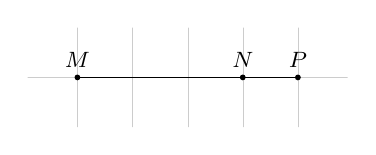
\begin{tikzpicture}[scale=0.7, font=\footnotesize, line join=round, line cap=round, >=stealth]
			\def\xt{-0.9} \def\xp{4.9} \def\yt{0.9} \def\yd{-0.9} % x_trái, x_phải, y_trên, y_dưới (giới hạn)
			\draw[line width=0.1pt,gray!40] (\xt,\yd) grid (\xp,\yt); % Lưới toạ độ
			\draw (\xt+0.9,0)--(\xp-0.9,0);
			\clip (\xt+0.1,\yd+0.1) rectangle (\xp-0.1,\yt-0.1);
			\draw (0,0)--(4,0);
			\foreach \x/\diem in {0/M,3/N,4/P}
			\fill (\x,0) circle (1.5pt) node[above]{$\diem$};
		\end{tikzpicture}
	\end{center}
	\choice
	{$\overrightarrow{MP}=4\overrightarrow{NP}$}
	{$\overrightarrow{PN}=-\dfrac{1}{3}\overrightarrow{MN}$}
	{\True $\overrightarrow{MN}=3\overrightarrow{PN}$}
	{$\overrightarrow{MN}=\dfrac{3}{4}\overrightarrow{MP}$}
	\loigiai{
		Từ hình vẽ và các phương án, ta thấy khẳng định sai là ``$\overrightarrow{MN}=3\overrightarrow{PN}$''.
	}
\end{ex}
\begin{ex}%[0H5N3-1]%[Dự án D - Đề cương 3 khối 10-11-12 NH25-26 - Nguyễn Tiến]%
	[\textit{Trích đề thi HKI - Trường THPT Nguyễn Gia Thiều, Hà Nội - Năm học 2024-2025}]
	Cho đoạn thẳng $AB$ và $M$ là một điểm nằm trên đoạn thẳng $AB$ sao cho $AM=\dfrac{1}{4}AB$. Khẳng định nào sau đây đúng?
	\choice
	{$\overrightarrow{AM}=-\dfrac{1}{4}\overrightarrow{AB}$}
	{\True $\overrightarrow{AM}=\dfrac{1}{4}\overrightarrow{AB}$}
	{$\overrightarrow{AB}=\dfrac{1}{4}\overrightarrow{AM}$}
	{$\overrightarrow{AB}=-\dfrac{1}{4}\overrightarrow{AM}$}
	\loigiai{
		Do $\overrightarrow{AM}$ và $\overrightarrow{AB}$ cùng chiều nên $\overrightarrow{AM}=\dfrac{1}{4}\overrightarrow{AB}$.
	}
\end{ex}
\begin{ex}%[0H5N3-1]%[Dự án D - Đề cương 3 khối 10-11-12 NH25-26 - Nguyễn Tiến]%
	[\textit{Trích đề thi GHKI - Trường THPT Lê Quý Đôn, Ninh Thuận - Năm học 2024-2025}]
	Cho hình chữ nhật $ABCD$ có $M$, $N$ lần lượt là trung điểm của $AB$, $BC$. Giá trị $k$ thỏa $\left|\overrightarrow{BD}\right|= k\left|\overrightarrow{MN}\right|$ là
	\choice
	{\True $2$}
	{$\dfrac{1}{2}$}
	{$3$}
	{$\dfrac{2}{3}$}
	\loigiai{
		Ta có $M$, $N$ là đường trung bình của $\triangle ABC$ nên $\left|\overrightarrow{B D}\right|=\left|\overrightarrow{AC}\right|=2\left|\overrightarrow{M N}\right|$.\\
		Suy ra $k=2$.
	}
\end{ex}
\begin{ex}%[0H5N3-1]%[Dự án D - Đề cương 3 khối 10-11-12 NH25-26 - Nguyễn Tiến]%
	[\textit{Trích đề thi HKI - Trường THPT Chu Văn An, Hà Nội - Năm học 2023-2024}]
	\immini{
		Cho đoạn thẳng $AB$ và $M$ là một điểm trên đoạn $AB$ sao cho $AM = \dfrac{1}{4}AB$. Trong các khẳng định sau, khẳng định nào đúng?
	}{
		\begin{tikzpicture}[scale=0.7, font=\footnotesize, line join=round, line cap=round, >=stealth]
			\coordinate (A) at (0,0);
			\coordinate (B) at (8,0);
			\coordinate (M) at ($(A)!0.25!(B)$);
			\draw[name path=AB] (A)--(B);
			\foreach \i/\g in {A/-90,B/-90,M/-90}{\draw[fill=black](\i) circle (1pt) ($(\i)+(\g:3mm)$) node[scale=1]{$\i$};}
			\foreach \x in {4,6}
				\fill (\x,0) circle (1.2pt);
		\end{tikzpicture}
	}
	\choice
	{\True $\overrightarrow{MA}=-\dfrac{1}{4}\overrightarrow{AB}$}
	{$\overrightarrow{MB}=\dfrac{1}{4}\overrightarrow{AB}$}
	{$\overrightarrow{MA}=\dfrac{1}{5}\overrightarrow{AB}$}
	{$\overrightarrow{MA}=-\dfrac{1}{5}\overrightarrow{AB}$}
	\loigiai{
		Ta có $AM = \dfrac{1}{4}AB \Rightarrow \overrightarrow{MA}=-\dfrac{1}{4}\overrightarrow{AB}$.
	}
\end{ex}
\begin{ex}%[0H5N3-1]%[Dự án D - Đề cương 3 khối 10-11-12 NH25-26 - Nguyễn Tiến]%
	[\textit{Trích đề thi HKI - Trường THPT Chu Văn An, Hà Nội - Năm học 2023-2024}]
	Cho hình thang $MNPQ$, $MN\parallel PQ$, $MN=2PQ$. Phát biểu nào sau đây đúng?
	\choice
	{$\overrightarrow{MN}=2\overrightarrow{PQ}$}
	{\True $\overrightarrow{MN}=-2\overrightarrow{PQ}$}
	{$\overrightarrow{MQ}=-2\overrightarrow{NP}$}
	{$\overrightarrow{MQ}=2\overrightarrow{NP}$}
	\loigiai{
		\immini{
			Ta có $MNPQ$ là hình thang.\\
			$\Rightarrow MN\parallel PQ$ và $MN=2PQ$.\\
			Vậy $\overrightarrow{MN}=-2\overrightarrow{PQ}$.
		}{
			\begin{tikzpicture}[scale=0.7, font=\footnotesize, line join=round, line cap=round, >=stealth]
				\coordinate (Q) at (0.5,2);
				\coordinate (P) at (2.5,2);
				\coordinate (M) at (0,0);
				\coordinate (N) at (4,0);
				\draw(M)--(N)--(P)--(Q)--cycle;
				\foreach \i/\g in {P/90,Q/90,M/-90,N/-90}{\draw[fill=white](\i) circle (1pt) ($(\i)+(\g:3mm)$) node[scale=1]{$\i$};}
			\end{tikzpicture}
		}	
	}
\end{ex}
\begin{ex}%[0H5N3-1]%[Dự án D - Đề cương 3 khối 10-11-12 NH25-26 - Nguyễn Tiến]%
	[\textit{Trích đề thi HKI - Trường THPT Chuyên Hùng Vương, Phú Thọ - Năm học 2023-2024}]
	Cho $\overrightarrow{AB}=2\overrightarrow{AC}$. Trong các khẳng định sau, có bao nhiêu khẳng định đúng?
	\begin{enumerate}
		\item Hai véc-tơ $\overrightarrow{AB}$ và $\overrightarrow{AC}$ cùng hướng.
		\item $A$, $B$, $C$ thẳng hàng và điểm $B$ nằm giữa $A$ và $C$.
		\item $A$, $B$, $C$ thẳng hàng và điểm $C$ nằm giữa $A$ và $B$.
	\end{enumerate}
	\choice
	{\True $2$}
	{$1$}
	{$3$}
	{$0$}
	\loigiai{
		Để giải câu hỏi này, ta cần xem xét từng khẳng định
		\begin{enumerate}
			\item Đúng, vì nếu $\overrightarrow{AB}=2\overrightarrow{AC}$ thì chúng có cùng hướng.
			\item Sai, vì $AB=2AC$ nên $B$ không nằm giữa $A$ và $C$.
			\item Đúng, vì nếu $\overrightarrow{AB}=2\overrightarrow{AC}$ thì $C$ nằm giữa $A$ và $B$.
		\end{enumerate}
		Vậy có $2$ khẳng định đúng.
	}
\end{ex}
\begin{ex}%[0H5N3-1]%[Dự án D - Đề cương 3 khối 10-11-12 NH25-26 - Nguyễn Tiến]%
	[\textit{Trích đề thi HKI - Trường THPT Nguyễn Khuyến, TPHCM - Năm học 2023-2024}]
	\immini{
		Đẳng thức nào sau đây mô tả đúng hình vẽ bên?
		\choice
		{$\overrightarrow{B I}+3 \overrightarrow{B A}=\overrightarrow{0}$}
		{$3 \overrightarrow{I A}+\overrightarrow{I B}=\overrightarrow{0}$}
		{$\overrightarrow{A I}+3 \overrightarrow{A B}=\overrightarrow{0}$}
		{\True $3 \overrightarrow{A I}+\overrightarrow{A B}=\overrightarrow{0}$}
	}{
		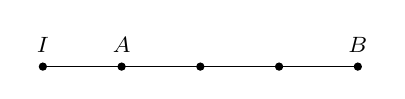
\begin{tikzpicture}[scale=1, font=\footnotesize, line join=round, line cap=round, >=stealth]
			\fill[black] (0,0)node[shift={(90:8pt)}]{$I$} circle (1.5pt);
			\fill[black] (1,0)node[shift={(90:8pt)}]{$A$} circle (1.5pt);
			\fill[black] (2,0) circle (1.5pt);
			\fill[black] (3,0) circle (1.5pt);
			\fill[black] (4,0)node[shift={(90:8pt)}]{$B$} circle (1.5pt);
			\draw (0,0) -- (4,0);
		\end{tikzpicture}
	}
	\loigiai{
		Ta có $\heva{& AB=3AI\\& \overrightarrow{AI} \text{ ngược hướng }\overrightarrow{AB}} \Rightarrow \overrightarrow{AB}=-3\overrightarrow{AI}$.\\
		Vậy $3 \overrightarrow{A I}+\overrightarrow{A B}=\overrightarrow{0}$.
	}
\end{ex}
\begin{ex}%[0H5N3-2]%[Dự án D - Đề cương 3 khối 10-11-12 NH25-26 - Nguyễn Tiến]%
	[\textit{Trích đề thi HKI - Trường THPT Chu Văn An, Hà Nội - Năm học 2023-2024}]
	Cho ba điểm phân biệt $A$, $B$, $C$. Nếu $\overrightarrow{AB}=-3\overrightarrow{AC}$ thì đẳng thức nào dưới đây đúng?
	\choice
	{$\overrightarrow{BC}=2\overrightarrow{AC}$}
	{$\overrightarrow{BC}=-2\overrightarrow{AC}$}
	{$\overrightarrow{BC}=-4\overrightarrow{AC}$}
	{\True $\overrightarrow{BC}=4\overrightarrow{AC}$}
	\loigiai{
		Ta có $\overrightarrow{AB}=-3\cdot\overrightarrow{AC}\Leftrightarrow \overrightarrow{AB} -\overrightarrow{AC}=-4\cdot\overrightarrow{AC}\Leftrightarrow\overrightarrow{CB} =-4\cdot\overrightarrow{AC}\Leftrightarrow\overrightarrow{BC} =4\cdot\overrightarrow{AC}$.
	}
\end{ex}
\begin{ex}%[0H5N3-2]%[Dự án D - Đề cương 3 khối 10-11-12 NH25-26 - Nguyễn Tiến]%
	[\textit{Trích đề thi HKI - Trường THPT Chuyên Hùng Vương, Phú Thọ - Năm học 2023-2024}]
	Cho $\overrightarrow{u}=2\overrightarrow{a}-3\big(\overrightarrow{a}-\overrightarrow{b}\big)+\overrightarrow{a}$. Khẳng định nào sau đây đúng?
	\choice
	{$\overrightarrow{u}=-3\overrightarrow{b}$}
	{$\overrightarrow{u}=6\overrightarrow{a}$}
	{$\overrightarrow{u}=-2\overrightarrow{a}+3\overrightarrow{b}$}
	{\True $\overrightarrow{u}=3\overrightarrow{b}$}
	\loigiai{
		Ta có $\overrightarrow{u}=2\overrightarrow{a}-3\big(\overrightarrow{a}-\overrightarrow{b}\big)+\overrightarrow{a}=2\overrightarrow{a}-3\overrightarrow{a}+3\overrightarrow{b}+\overrightarrow{a}=3\overrightarrow{b}$.
	}
\end{ex}
\begin{ex}%[0H5N3-3]%[Dự án D - Đề cương 3 khối 10-11-12 NH25-26 - Nguyễn Tiến]%
	[\textit{Trích đề thi HKI - Trường THPT Nguyễn Công Trứ, TPHCM - Năm học 2023-2024}]
	Cho ba điểm $M$, $N$, $P$ phân biệt thỏa mãn $\overrightarrow{MN} = -3\overrightarrow{MP}$. Hình vẽ nào sau đây biểu diễn vị trí tương đối của ba điểm đã cho?
	\begin{center}
		\begin{tikzpicture}[scale=0.7, font=\footnotesize, line join=round, line cap=round, >=stealth]
			\path (0,0) coordinate (M) node[below]{$M$}
			(-1,-3) coordinate (P) node[below]{$P$}
			(-3,0) coordinate (N) node[below]{$N$};					
			\foreach \x in {(M),(N),(P)}{\draw[fill=black] \x circle (0.05) ;}
			\draw (-1,-3.4) node[below]{$\text{Hình 1}$};
		\end{tikzpicture} \qquad\qquad
		\begin{tikzpicture}[scale=0.6, font=\footnotesize, line join=round, line cap=round, >=stealth]
			\path (3,1) coordinate (N) node[below]{$N$}
			(0,-2) coordinate (M) node[below]{$M$}
			(-1,-3) coordinate (P) node[below]{$P$};					
			\draw (N)--(P);
			\foreach \x in {(M),(N),(P)}{\draw[fill=black] \x circle (0.05) ;}
			\draw (1,-3.4) node[below]{$\text{Hình 2}$};
		\end{tikzpicture} \qquad\qquad
		\begin{tikzpicture}[scale=0.7, font=\footnotesize, line join=round, line cap=round, >=stealth]
			\path 
			(0,-2) coordinate (N) node[below]{$N$}
			(-3,1) coordinate (M) node[below]{$M$}
			(-2,0) coordinate (P) node[below]{$P$};			
			\draw (N)--(M);
			\foreach \x in {(M),(N),(P)}{\draw[fill=black] \x circle (0.05) ;}
			\draw (-1,-2.4) node[below]{$\text{Hình 3}$};
		\end{tikzpicture} \qquad\qquad
		\begin{tikzpicture}[scale=0.7, font=\footnotesize, line join=round, line cap=round, >=stealth]
			\path 
			(-1,-2) coordinate (N) node[below]{$N$}
			(2,1) coordinate (M) node[below]{$M$}
			(3,0) coordinate (P) node[below]{$P$};			
			\draw (N)--(M)--(P);
			\foreach \x in {(M),(N),(P)}{\draw[fill=black] \x circle (0.05) ;}
			\draw (2,-2.4) node[below]{$\text{Hình 4}$};
		\end{tikzpicture}
	\end{center}
	\choice
	{Hình $3$}
	{\True Hình $2$}
	{Hình $1$}
	{Hình $4$}
	\loigiai{
		Hình $2$ biểu diễn vị trí tương đối của ba điểm đã cho.
	}
\end{ex}
\begin{ex}%[0H5N3-4]%[Dự án D - Đề cương 3 khối 10-11-12 NH25-26 - Nguyễn Tiến]%
	[\textit{Trích đề thi HKI - Trường THPT Nguyễn Văn Trỗi, Khánh Hoà - Năm học 2023-2024}]
	Cho năm điểm $E$, $F$, $G$, $H$ và $I$ thẳng hàng như hình vẽ.
	\begin{center}
		\begin{tikzpicture}[>=stealth,line join=round,line cap=round,font=\footnotesize,scale=0.8]
			\path 
			(0,0) coordinate (a)
			(14,0) coordinate (b)
			($(a)!1/14!(b)$) coordinate (E)
			($(a)!2/14!(b)$) coordinate (A)
			($(a)!3/14!(b)$) coordinate (B)
			($(a)!3/14!(b)$) coordinate (C)
			($(a)!4/14!(b)$) coordinate (D)
			($(a)!5/14!(b)$) coordinate (F)
			($(a)!6/14!(b)$) coordinate (E1)
			($(a)!7/14!(b)$) coordinate (E2)
			($(a)!8/14!(b)$) coordinate (E3)
			($(a)!9/14!(b)$) coordinate (E4)
			($(a)!10/14!(b)$) coordinate (G)
			($(a)!11/14!(b)$) coordinate (H)
			($(a)!12/14!(b)$) coordinate (E5)
			($(a)!13/14!(b)$) coordinate (I)
			;
			\draw (a)--(b);
			\foreach \x/\y in {E/-90,F/-90,G/-90,H/-90,I/-90}
			\draw[fill=black] (\x) circle (1.1pt) + (\y:0.5cm) node{$\x$};
			\foreach \x/\y in {E1/-90,E2/-90,E3/-90,E4/-90,E5/-90,A/0,B/0,C/0,D/0}
			\draw[fill=black] (\x) circle (1.1pt) + (\y:0.5cm) ;
		\end{tikzpicture}
	\end{center}
	Khẳng định nào sau đây đúng?
	\choice
	{$\overrightarrow{E F}=\dfrac{4}{3} \overrightarrow {IG}$}
	{$\overrightarrow{H I}=\dfrac{1}{4} \overrightarrow{I F}$}
	{\True $\overrightarrow{G I}=-\dfrac{3}{8} \overrightarrow{I F}$}
	{$\overrightarrow{F G}=-\dfrac{5}{4} \overrightarrow{E F}$}
	\loigiai{
		Theo hình vẽ $\overrightarrow{GI}$ và $\overrightarrow{IF}$ ngược hướng và $8FI=3GI$.\\
		Do đó  $\overrightarrow{G I}=-\dfrac{3}{8} \overrightarrow{I F}$.
	}
\end{ex}
\begin{ex}%[0H5H3-1]%[Dự án D - Đề cương 3 khối 10-11-12 NH25-26 - Nguyễn Tiến]%
	[\textit{Trích đề thi HKI - Trường THPT Chuyên Lê Khiết, Quảng Ngãi - Năm học 2023-2024}]
	Trên đường thẳng $M N$ lấy $P$ sao cho $\overrightarrow{M N}=-4 \overrightarrow{N P}$. Điểm $P$ được xác định đúng trong hình vẽ nào sau đây?
	\begin{center}
		\begin{tabular}{ccc}
			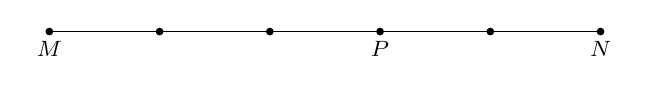
\begin{tikzpicture}[scale=0.7, font=\footnotesize, line join=round, line cap=round, >=stealth]
				\coordinate [label=below:$M$](M) at (0,0);
				\coordinate [label=below:$P$](P) at (6,0);
				\coordinate [label=below:$N$](N) at (10,0);
				\coordinate (A) at (2,0);
				\coordinate (B) at (4,0);
				\coordinate (C) at (8,0);
				\foreach \diem in {P,M,N,A,B,C}	\fill (\diem)circle(2pt);		
				\draw[smooth](M)--(N);
			\end{tikzpicture}&\hspace*{2cm}&
			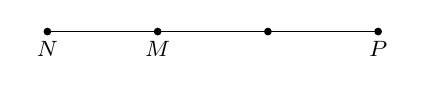
\begin{tikzpicture}[scale=0.7, font=\footnotesize, line join=round, line cap=round, >=stealth]
				\coordinate [label=below:$M$](M) at (2,0);
				\coordinate [label=below:$P$](P) at (6,0);
				\coordinate [label=below:$N$](N) at (0,0);
				\coordinate (A) at (4,0);
				\foreach \diem in {P,M,N,A}	\fill (\diem)circle(2pt);		
				\draw[smooth](P)--(N);
			\end{tikzpicture}\\
			Hình 1&& Hình 2\\
			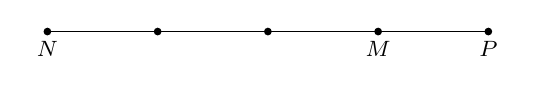
\begin{tikzpicture}[scale=0.7, font=\footnotesize, line join=round, line cap=round, >=stealth]
				\coordinate [label=below:$M$](M) at (6,0);
				\coordinate [label=below:$P$](P) at (8,0);
				\coordinate [label=below:$N$](N) at (0,0);
				\coordinate (A) at (2,0);
				\coordinate (B) at (4,0);
				\foreach \diem in {P,M,N,A,B}	\fill (\diem)circle(2pt);		
				\draw[smooth](P)--(N);
			\end{tikzpicture}&\hspace*{2cm}&
			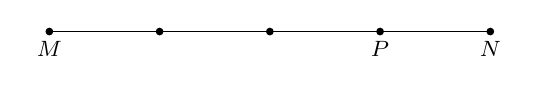
\begin{tikzpicture}[scale=0.7, font=\footnotesize, line join=round, line cap=round, >=stealth]
				\coordinate [label=below:$M$](M) at (0,0);
				\coordinate [label=below:$P$](P) at (6,0);
				\coordinate [label=below:$N$](N) at (8,0);
				\coordinate (A) at (4,0);
				\coordinate (B) at (2,0);
				\foreach \diem in {P,M,N,A,B}	\fill (\diem)circle(2pt);		
				\draw[smooth](M)--(N);
			\end{tikzpicture}\\
			Hình 3&& Hình 4
		\end{tabular}
	\end{center}
	\choice
	{Hình $1$}
	{\True Hình $4$}
	{Hình $3$}
	{Hình $2$}
	\loigiai{
		Vì $\overrightarrow{M N}=-4 \overrightarrow{N P}$ nên $\overrightarrow{M N}$ ngược hướng với $ \overrightarrow{N P}$ và $MN=4N P$.\\
		Vậy $P$ nằm giữa $MN$ và chia $MN$ theo tỉ lệ $\dfrac{1}{4}$. 
	}
\end{ex}
\begin{ex}%[0H5H3-1]%[Dự án D - Đề cương 3 khối 10-11-12 NH25-26 - Nguyễn Tiến]%
	[\textit{Trích đề thi HKI - Trường THPT Hùng Vương, TPHCM - Năm học 2023-2024}]
	\immini{
		Cho tam giác $ABC$ có trọng tâm $G$, gọi $D$ là trung điểm của cạnh $BC$.
		Khẳng định nào sau đây \textbf{sai}?
		\choice
		{$\overrightarrow{BC}=2 \overrightarrow{DC}$}
		{\True $\overrightarrow{GA}=2 \overrightarrow{GD}$}
		{$\overrightarrow{GD}=-\dfrac{1}{3}\overrightarrow{DA}$}
		{$\overrightarrow{AD}=3 \overrightarrow{GD}$}
	}{
		\begin{tikzpicture}[scale=0.7, font=\footnotesize, line join=round, line cap=round, >=stealth]
			\def\a{3}
			\def\b{5}
			\def\g{-120}
			\draw (0,0) coordinate (A)--++(\g:\a) coordinate (B)--++(0:\b) coordinate (C)--cycle;
			\path (barycentric cs:C=1,B=1)coordinate(D);
			\path (barycentric cs:A=1,B=1,C=1)coordinate(G);
			\foreach \x/\g in {A/90,B/180,C/0,G/0,D/-90}
			\fill (\x) circle (1pt)($(\x)+(\g:3mm)$) node{$\x$};
			\draw (A)--(D);
			% \draw[->] (B')--(B); 
			% \draw[->] (A)--(G);
		\end{tikzpicture}	
	}
	\loigiai{
		Hai $\overrightarrow{GA}$ và $\overrightarrow{GD}$ ngược hướng nên  mệnh đề $\overrightarrow{GA}=2 \overrightarrow{GD}$ sai.
	}
\end{ex}
\begin{ex}%[0H5H3-2]%[Dự án D - Đề cương 3 khối 10-11-12 NH25-26 - Nguyễn Tiến]%
	[\textit{Trích đề thi HKI - Trường THPT Hồ Thị Bi, TPHCM - Năm học 2024-2025}]
	Cho hình chữ nhật $ABCD$ có $E$ là trung điểm $BC$. Khi đó $\overrightarrow{u}=\overrightarrow{BA}+2\overrightarrow{EC}$ bằng véc-tơ nào sau đây?
	\choice
	{$\overrightarrow{DB}$}
	{\True $\overrightarrow{BD}$}
	{$\overrightarrow{DE}$}
	{$\overrightarrow{AC}$}
	\loigiai{
		\immini{
			Ta có $\overrightarrow{u}=\overrightarrow{BA}+2\overrightarrow{EC}=\overrightarrow{BA}+\overrightarrow{BC}=\overrightarrow{BD}$.
		}{
			\begin{tikzpicture}[scale=0.7, font=\footnotesize, line join=round, line cap=round, >=stealth]
				\coordinate (A) at (0,3);
				\coordinate (B) at (5,3);
				\coordinate (D) at (0,0);
				\coordinate (C) at ($(B)+(D)-(A)$);
				\coordinate (E) at ($(B)!0.5!(C)$);
				\draw[->] (B)--(A);
				\draw[->] (B)--(C);
				\draw[->] (B)--(D);
				\draw(A)--(D) (C)--(D) (B)--(D);
				\foreach \i/\g in {A/90,B/90,C/-90,D/-90,E/0}{\draw[fill=black](\i) circle (1pt) ($(\i)+(\g:3mm)$) node[scale=1]{$\i$};}
			\end{tikzpicture}
		}
	}
\end{ex}
\begin{ex}%[0H5H3-2]%[Dự án D - Đề cương 3 khối 10-11-12 NH25-26 - Nguyễn Tiến]%
	[\textit{Trích đề thi HKI - Trường THPT Chuyên Trần Phú, Hải Phòng - Năm học 2023-2024}]
	Cho tam giác $ABC$ có trọng tâm $G$. Khẳng định nào sau đây là đúng?
	\choice
	{$\overrightarrow{BG}=\dfrac{2}{3}\overrightarrow{BA}+\dfrac{2}{3}\overrightarrow{BC}$}
	{\True $\overrightarrow{BG}=\dfrac{1}{3}\overrightarrow{BA}+\dfrac{1}{3}\overrightarrow{BC}$}
	{$\overrightarrow{BG}=\dfrac{2}{3}\overrightarrow{BA}+\dfrac{1}{3}\overrightarrow{BC}$}
	{$\overrightarrow{BG}=\dfrac{1}{3}\overrightarrow{BA}+\dfrac{2}{3}\overrightarrow{BC}$}
	\loigiai{
		Ta có $G$ là trọng tâm tam giác $ABC$ suy ra 
		\begin{eqnarray*}
			& & \overrightarrow{GA}+\overrightarrow{GB}+\overrightarrow{GC}=\overrightarrow{0}\\
			&\Leftrightarrow & 3\overrightarrow{GB}+\overrightarrow{BA}+\overrightarrow{BC}=\overrightarrow{0}\\
			&\Leftrightarrow & \overrightarrow{BA}+\overrightarrow{BC}=3\overrightarrow{BG}\\
			&\Leftrightarrow & \dfrac{1}{3}\overrightarrow{BA}+\dfrac{1}{3}\overrightarrow{BC}=\overrightarrow{BG}.
		\end{eqnarray*}
	}
\end{ex}
\begin{ex}%[0H5H3-3]%[Dự án D - Đề cương 3 khối 10-11-12 NH25-26 - Nguyễn Tiến]%
	[\textit{Trích đề thi HKI - Trường THPT Nguyễn Thái Bình, TPHCM - Năm học 2023-2024}]
	Trên đường thẳng $MN$ lấy điểm $P$ sao cho $\overrightarrow{MP}=3\overrightarrow{PN}$. Điểm $P$ được xác định \textbf{đúng} trong hình vẽ nào sau đây?
	\choice
	{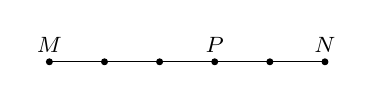
\begin{tikzpicture}[scale=0.7, font=\footnotesize, line join=round, line cap=round, >=stealth]
			\path 
			(0,0) coordinate (O) node[above]{$M$}
			(1,0) coordinate (A) 
			(2,0) coordinate (B)
			(3,0) coordinate (C)node[above]{$P$}
			(4,0) coordinate (D)
			(5,0) coordinate (E)  node[above]{$N$};
			\draw(O)--(E);
			\foreach \i in {O,A,B,C,D,E}{\draw[fill=black](\i) circle (1.5pt);}
	\end{tikzpicture}}
	{\True 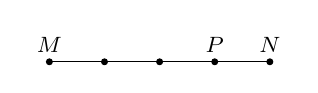
\begin{tikzpicture}[scale=0.7, font=\footnotesize, line join=round, line cap=round, >=stealth]
			\path 
			(0,0) coordinate (O) node[above]{$M$}
			(1,0) coordinate (A) 
			(2,0) coordinate (B)
			(3,0) coordinate (C) node[above]{$P$}
			(4,0) coordinate (D) node[above]{$N$};
			\draw(O)--(D);
			\foreach \i in {O,A,B,C,D}{\draw[fill=black](\i) circle (1.5pt);}
	\end{tikzpicture}}
	{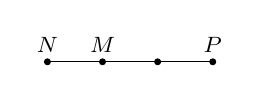
\begin{tikzpicture}[scale=0.7, font=\footnotesize, line join=round, line cap=round, >=stealth]
			\path 
			(0,0) coordinate (O) node[above]{$N$}
			(1,0) coordinate (A) node[above]{$M$}
			(2,0) coordinate (B)
			(3,0) coordinate (C) node[above]{$P$};
			\draw(O)--(C);
			\foreach \i in {O,A,B,C}{\draw[fill=black](\i) circle (1.5pt);}
	\end{tikzpicture}}
	{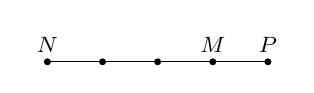
\begin{tikzpicture}[scale=0.7, font=\footnotesize, line join=round, line cap=round, >=stealth]
			\path 
			(0,0) coordinate (O) node[above]{$N$}
			(1,0) coordinate (A) 
			(2,0) coordinate (B)
			(3,0) coordinate (C) node[above]{$M$}
			(4,0) coordinate (D) node[above]{$P$};
			\draw(O)--(D);
			\foreach \i in {O,A,B,C,D}{\draw[fill=black](\i) circle (1.5pt);}
	\end{tikzpicture}}
	\loigiai{
		Ta có $\overrightarrow{MP}=3\overrightarrow{PN}$ nên suy ra hai véc-tơ $\overrightarrow{MP}$, $\overrightarrow{PN}$ cùng hướng và $MP=3PN$.\\
		Vậy phương án đúng là
		\begin{center}
			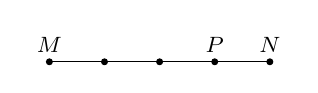
\begin{tikzpicture}[scale=0.7, font=\footnotesize, line join=round, line cap=round, >=stealth]
				\path 
				(0,0) coordinate (O) node[above]{$M$}
				(1,0) coordinate (A) 
				(2,0) coordinate (B) 
				(3,0) coordinate (C) node[above]{$P$}
				(4,0) coordinate (D) node[above]{$N$};
				\draw(O)--(D);
				\foreach \i in {O,A,B,C,D}{\draw[fill=black](\i) circle (1.5pt);}
			\end{tikzpicture}
		\end{center}
	}
\end{ex}
\begin{ex}%[0H5H3-4]%[Dự án D - Đề cương 3 khối 10-11-12 NH25-26 - Nguyễn Tiến]%
	[\textit{Trích đề thi GHKI - Trường THPT Cầu Giấy, Hà Nội - Năm học 2023-2024}]
	Cho đoạn thẳng $A B$ và $M$ là một điểm trong đoạn thẳng $A B$ sao cho $A M=\dfrac{1}{5}A B$. Tìm $k$ để $\overrightarrow{M A}=k \overrightarrow{M B}$.
	\choice
	{$k=\dfrac{1}{4}$}
	{$k=4$}
	{$k=-4$}
	{\True $k=-\dfrac{1}{4}$}
	\loigiai{
		Vì điểm $M$ thuộc đoạn thẳng $AB$ và $A M=\dfrac{1}{5}A B$ nên
		$$\overrightarrow{AM}=\dfrac{1}{5} \overrightarrow{AB} \Leftrightarrow -\overrightarrow{MA}=\dfrac{1}{5}\left(\overrightarrow{MB}-\overrightarrow{MA}\right) \Leftrightarrow \overrightarrow{MA}=-\dfrac{1}{4}\overrightarrow{MB}.$$ 
		Vậy $k=-\dfrac{1}{4}$.
	}
\end{ex}
\begin{ex}%[0H5H3-5]%[Dự án D - Đề cương 3 khối 10-11-12 NH25-26 - Nguyễn Tiến]%
	[\textit{Trích đề thi GHKI - Trường THPT Sóc Sơn, Hà Nội - Năm học 2023-2024}]
	Cho tam giác $ABC$, gọi $M$ là trung điểm của cạnh $BC$, $N$ là điểm trên cạnh $AB$ sao cho $AN=3NB$. Đẳng thức nào sau đây \textbf{đúng}? 
	\choice
	{$\overrightarrow{MN}=\dfrac{1}{4} \overrightarrow{AB}+\dfrac{1}{2} \overrightarrow{AC}$}
	{$\overrightarrow{MN}=\dfrac{1}{2} \overrightarrow{AB}-\dfrac{1}{4} \overrightarrow{AC}$}
	{$\overrightarrow{MN}=\dfrac{1}{2} \overrightarrow{AB}+\dfrac{1}{4} \overrightarrow{AC}$}
	{\True $\overrightarrow{MN}=\dfrac{1}{4} \overrightarrow{AB}-\dfrac{1}{2} \overrightarrow{AC}$}
	\loigiai{
		\immini{
			Ta có
			\begin{eqnarray*}
				\overrightarrow{MN}&=&\overrightarrow{MB}+\overrightarrow{BN}=\dfrac{1}{2}\overrightarrow{CB}+\dfrac{1}{4}\overrightarrow{BA}\\
				&=&\dfrac{1}{2}\left( \overrightarrow{AB}-\overrightarrow{AC} \right)-\dfrac{1}{4}\overrightarrow{AB}\\
				&=&\dfrac{1}{4}\overrightarrow{AB}-\dfrac{1}{2}\overrightarrow{AC}.
			\end{eqnarray*}
		}{
			\begin{tikzpicture}[scale=1, font=\footnotesize, line join=round, line cap=round, >=stealth]
				\def\r{3}
				\path 	(180:\r) coordinate (B)
				(0:\r) coordinate (C)	
				(130:\r) coordinate (A)
				($(B)!1/2!(C)$) coordinate (M)
				($(A)!3/4!(B)$) coordinate (N);
				\draw (A)--(B)--(C)--cycle	(M)--(N);
				\foreach \x/ \goc in {A/135,B/-135,C/-45,M/-90,N/180} 
				\fill (\x) circle (1pt)
				($(\x)+(\goc:3mm)$) node {$\x$};	
			\end{tikzpicture}
		}
	}
\end{ex}
\begin{ex}%[0H5H3-5]%[Dự án D - Đề cương 3 khối 10-11-12 NH25-26 - Nguyễn Tiến]%
	[\textit{Trích đề thi HKI - Trường THPT Nguyễn Gia Thiều, Hà Nội - Năm học 2023-2024}]
	Biết tam giác $ABC$ có $AM$ là đường trung tuyến và $G$ là trọng tâm. Khẳng định nào sau đây đúng?
	\choice
	{$\overrightarrow{GM}=\dfrac{1}{3}\overrightarrow{AB}+\dfrac{1}{3}\overrightarrow{AC}$}
	{$\overrightarrow{GM}=\dfrac{1}{3}\overrightarrow{AB}+\dfrac{1}{2}\overrightarrow{AC}$}
	{\True $\overrightarrow{GM}=\dfrac{1}{6}\overrightarrow{AB}+\dfrac{1}{6}\overrightarrow{AC}$}
	{$\overrightarrow{GM}=\dfrac{2}{3}\overrightarrow{AB}+\dfrac{2}{3}\overrightarrow{AC}$}
	\loigiai{
		\immini{
			Ta có $\overrightarrow{GM}=\dfrac{1}{3}\overrightarrow{AM} =\dfrac{1}{3}\cdot\dfrac{1}{2}\left(\overrightarrow{AB}+\overrightarrow{AC}\right) =\dfrac{1}{6}\overrightarrow{AB}+\dfrac{1}{6}\overrightarrow{AC}$.
		}{
			\begin{tikzpicture}[scale=0.5, font=\footnotesize, line join=round, line cap=round, >=stealth]
				\path (0,0) coordinate (B)
				(2,5) coordinate (A)
				(6,0) coordinate (C)
				($(B)!0.5!(C)$) coordinate (M)
				($(A)!{2/3}!(M)$) coordinate (G)
				;
				\draw (M)--(A)--(B)--(C)--(A);
				\foreach \p / \r in {A/90,B/-135,C/-45,M/-90,G/45}
				\fill (\p) circle (1.2pt) node[shift={(\r:3mm)}]{$\p$};
			\end{tikzpicture}
		}
	}
\end{ex}
\Closesolutionfile{ans}
%=================

\ind{PHẦN II.} \inden{Câu trắc nghiệm đúng sai. Trong mỗi ý a), b), c), d) ở mỗi câu, học sinh chọn đúng hoặc sai.}\\
\setcounter{ex}{0}
\Opensolutionfile{ans}[ans/0H5-Bai3-DS]%--Đặt tên 0H5-Bai3-DS
\begin{ex}%[0H5V3-5]%[Dự án D - Đề cương 3 khối 10-11-12 NH25-26 - Nguyễn Tiến]%
	[\textit{Trích đề thi GHKI - Trường THPT Chuyên Lê Hồng Phong, TPHCM - Năm học 2024-2025}]
	Cho tam giác $ABC$ có $G$ là trọng tâm và $I$ là trung điểm của đoạn thẳng $BC$. Đặt $\overrightarrow{AB}=\overrightarrow{a}$, $\overrightarrow{AC}=\overrightarrow{b}$.
	\choiceTF
	{\True $\overrightarrow{AI}=\dfrac{1}{2} \overrightarrow{a}+\dfrac{1}{2} \overrightarrow{b}$}
	{$\overrightarrow{IG}=-\dfrac{1}{6} \overrightarrow{a}+\dfrac{1}{6} \overrightarrow{b}$}
	{\True $\overrightarrow{BI}=-\dfrac{1}{2} \overrightarrow{a}+\dfrac{1}{2} \overrightarrow{b}$}
	{\True $\overrightarrow{CI}=\dfrac{1}{2} \overrightarrow{a}-\dfrac{1}{2} \overrightarrow{b}$}
	\loigiai{
		\immini{
			\begin{itemchoice}
				\itemch Ta có $\overrightarrow{AI}=\dfrac{1}{2} \overrightarrow{AB}+\dfrac{1}{2} \overrightarrow{AC}=\dfrac{1}{2} \overrightarrow{a}+\dfrac{1}{2} \overrightarrow{b}$.
				\itemch Ta có $\overrightarrow{IG}=-\dfrac{1}{3}\overrightarrow{AI}=-\dfrac{1}{6} \overrightarrow{a}-\dfrac{1}{6} \overrightarrow{b}$.
				\itemch Ta có $\overrightarrow{BI}=\overrightarrow{AI}-\overrightarrow{AB}=-\dfrac{1}{2} \overrightarrow{a}+\dfrac{1}{2} \overrightarrow{b}$.
				\itemch Ta có $\overrightarrow{CI}=-\overrightarrow{BI}=\dfrac{1}{2} \overrightarrow{a}-\dfrac{1}{2} \overrightarrow{b}$.
			\end{itemchoice}
		}{
			\begin{tikzpicture}[scale=0.7, font=\footnotesize, line join=round, line cap=round, >=stealth]
				\draw[->] (1,3)node [above]{$A$}--(0,0) node [below]{$B$};
				\coordinate[label=left:$\overrightarrow{a}$] (a) at ($(A)!0.5!(B)$);
				\coordinate[label=right:$\overrightarrow{b}$] (b) at ($(A)!0.5!(C)$);
				\draw[->] (1,3)--(5,0) node [below]{$C$};
				\draw (1,3)--(2.5,0) node [below]{$I$} (0,0)--(5,0);
				\node at (2,1) [right]{$G$};
				\foreach \x/\y in {1/3,0/0,5/0,2/1,2.5/0}
					\fill (\x,\y) circle (1.2pt);
			\end{tikzpicture}
		}
	}
\end{ex}
\begin{ex}%[0H5H3-5]%[Dự án D - Đề cương 3 khối 10-11-12 NH25-26 - Nguyễn Tiến]%
	[\textit{Trích đề thi GHKI - Trường THPT Nguyễn Thị Minh Khai, TPHCM - Năm học 2024-2025}]
	Cho hình bình hành $ABCD$ có tâm $O$, $G$ là trọng tâm tam giác $ABC$ và $N$ là trung điểm $AB$.
	\choiceTF
	{$\overrightarrow{BO} + \overrightarrow{OD} = \overrightarrow{0}$}
	{\True $\overrightarrow{AB} + \overrightarrow{AD} = \overrightarrow{AC}$}
	{$\overrightarrow{BG} = \dfrac{2}{3}\left(\overrightarrow{BA} + \overrightarrow{BC} \right)$}
	{\True Nếu $\overrightarrow{AB} = x\overrightarrow{BO} + y\overrightarrow{CN}$ thì $x + y = -2$}
	\loigiai{
		\begin{itemchoice}
			\immini{
				\itemch Ta có $\overrightarrow{BO} + \overrightarrow{OD} = \overrightarrow{BD}$.\\
				Mà $B$, $D$ là hai điểm phân biệt trên hình bình hành $ABCD$ nên $\overrightarrow{BD} \neq \overrightarrow{0}$.\\
				Do đó $\overrightarrow{BO} + \overrightarrow{OD} \neq \overrightarrow{0}$.
				\itemch Xét hình bình hành $ABCD$, áp dụng quy tắc hình bình hành, ta có $$\overrightarrow{AB} + \overrightarrow{AD} = \overrightarrow{AC}.$$
				\itemch Vì $O$ là tâm của hình bình hành $ABCD$ nên $O$ là trung điểm của $AC$.\\
				Khi đó, ta có $\overrightarrow{BA} + \overrightarrow{BC} = 2\overrightarrow{BO} + \left(\overrightarrow{OA} + \overrightarrow{OC}\right) = 2\overrightarrow{BO} + \overrightarrow{0} = 2\overrightarrow{BO}$.\\
				Suy ra $\overrightarrow{BO} = \dfrac{1}{2}\left(\overrightarrow{BA} + \overrightarrow{BC}\right)$.\\
				Vì $G$ là trọng tâm $\triangle ABC$ nên
				$$\overrightarrow{BG} = \dfrac{2}{3}\overrightarrow{BO} = \dfrac{2}{3}\cdot \dfrac{1}{2}\left(\overrightarrow{BA} + \overrightarrow{BC}\right) = \dfrac{1}{3}\left(\overrightarrow{BA} + \overrightarrow{BC}\right).$$
				\itemch Ta có
				\allowdisplaybreaks
				\begin{eqnarray*}
					\overrightarrow{BO} + \overrightarrow{CN} &=& \overrightarrow{BA} + \overrightarrow{AO} + \overrightarrow{CA} + \overrightarrow{AN} = -\overrightarrow{AB} + \dfrac{1}{2}\overrightarrow{CA} + \dfrac{1}{2}\overrightarrow{AB}\\
					&=& -\dfrac{1}{2}\overrightarrow{AB} + \dfrac{1}{2}\left(\overrightarrow{CN} + \overrightarrow{NA}\right) = -\dfrac{1}{2}\overrightarrow{AB} + \dfrac{1}{2}\left(\overrightarrow{CN} + \dfrac{1}{2}\overrightarrow{BA}\right)\\
					&=& -\dfrac{3}{4}\overrightarrow{AB} + \dfrac{1}{2}\overrightarrow{CN}.
				\end{eqnarray*}
				Do đó $\dfrac{3}{4}\overrightarrow{AB}= -\overrightarrow{BO} - \dfrac{1}{2}\overrightarrow{CN} \Leftrightarrow \overrightarrow{AB} = -\dfrac{4}{3}\overrightarrow{BO} - \dfrac{2}{3}\overrightarrow{CN}$.\\
				Vậy $x = -\dfrac{4}{3}$ và $y = -\dfrac{2}{3}$, suy ra $x + y = -\dfrac{4}{3} + \left( -\dfrac{2}{3}\right) = -2$.
			}{
				\begin{tikzpicture}[scale=0.7, font=\footnotesize, line join=round, line cap=round, >=stealth]
					\path 
					(0,0) coordinate (A)
					(-1,-2) coordinate (B)
					(2.5,-2) coordinate (C)
					($(A)-(B)+(C)$) coordinate (D)
					($(A)!0.5!(B)$) coordinate (N)
					($(A)!0.5!(C)$) coordinate (O)
					($(B)!2/3!(O)$) coordinate (G)
					;
					\draw 
					(A)--(B)--(C)--(D)--(A)--(C)--(N) (B)--(D);
					\foreach \p/\g in {B/-90, D/90, A/90, C/-90,N/180,G/-90,O/80}
					\draw[fill=black] (\p) circle (1pt) node[shift=(\g:3mm)] {$\p$};
				\end{tikzpicture}
			}
		\end{itemchoice}
	}
\end{ex}
\begin{ex}%[0H5H3-7]%[Dự án D - Đề cương 3 khối 10-11-12 NH25-26 - Nguyễn Tiến]%
	[\textit{Trích đề thi HKI - Trường THPT Hồ Thị Bi, TPHCM - Năm học 2024-2025}]
	\immini{
		Cho tam giác $ABC$ đều có cạnh bằng $a$. Gọi $I$ là trung điểm cạnh $BC$.
		\choiceTF
		{\True $\overrightarrow{BC}=2\overrightarrow{BI}$}
		{Tập hợp các điểm $M$ thỏa mãn $\overrightarrow{MB}-\overrightarrow{MC}=\overrightarrow{BM}-\overrightarrow{BA}$ là đường thẳng đi qua $A$ và song song với $BC$}
		{\True $\left|\overrightarrow{BI}+\overrightarrow{CI}+2\overrightarrow{AI}\right|=a\sqrt{3}$}
		{$\left|\overrightarrow{AI}+\overrightarrow{BC}\right|=2a$}
	}{
		\begin{tikzpicture}[scale=0.6, font=\footnotesize, line join=round, line cap=round, >=stealth]
			\def\canh{5}
			\coordinate (B) at (0,0);
			\coordinate (C) at (\canh,0);
			\coordinate (A) at ($(B) + (60:\canh)$);
			\coordinate (I) at ($(B)!0.5!(C)$);
			\draw(A)--(B)--(C)--cycle;
			\path (A)--(B) node[midway,sloped,scale=0.5]{$|$};
			\path (A)--(C) node[midway,sloped,scale=0.5]{$|$};
			\foreach \i/\g in {A/90,B/-90,C/-90,I/-90}{\draw[fill=black](\i) circle (1pt) ($(\i)+(\g:3mm)$) node[scale=1]{$\i$};}
		\end{tikzpicture}
	}
	\loigiai{
		\begin{center}
			\begin{tikzpicture}[scale=0.5, font=\footnotesize, line join=round, line cap=round, >=stealth]
				\def\canh{5}
				\coordinate (B) at (0,0);
				\coordinate (C) at (\canh,0);
				\coordinate (A) at ($(B) + (60:\canh)$);
				\coordinate (I) at ($(B)!0.5!(C)$);
				\coordinate (N) at ($(C)!-1!(I)$);
				\draw(A)--(B)--(C)--cycle (A)--(I) (A)--(N)--(C);
				\path (A)--(B) node[midway,sloped,scale=0.5]{$|$};
				\path (A)--(C) node[midway,sloped,scale=0.5]{$|$};
				\foreach \i/\g in {A/90,B/-90,C/-90,I/-90,N/-90}{\draw[fill=black](\i) circle (1pt) ($(\i)+(\g:3mm)$) node[scale=1]{$\i$};}
			\end{tikzpicture}
		\end{center}
		\begin{itemchoice}
			\itemch Ta có $\overrightarrow{BC}$ và $\overrightarrow{BI}$ cùng hướng, $BC=2BI$ nên $\overrightarrow{BC}=2\overrightarrow{BI}$.
			\itemch Ta có $\overrightarrow{MB}-\overrightarrow{MC}=\overrightarrow{BM}-\overrightarrow{BA} \Rightarrow \overrightarrow{CB}=\overrightarrow{AM}$.\\
			Vậy $M$ là điểm sao cho $ACBM$ là hình bình hành.
			\itemch Do $\overrightarrow{BI}+\overrightarrow{CI}=\overrightarrow{0}$ nên ta có
			\[\left|\overrightarrow{BI}+\overrightarrow{CI}+2\overrightarrow{AI}\right|=\left|2\overrightarrow{AI}\right|=2\left|\overrightarrow{AI}\right|=2\cdot \dfrac{a\sqrt{3}}{2}=a\sqrt{3}.\]
			\itemch Gọi $N$ là điểm sao cho $\overrightarrow{IN}=\overrightarrow{BC}$. \\
			Ta có $\left|\overrightarrow{AI}+\overrightarrow{BC}\right|=\left|\overrightarrow{AI}+\overrightarrow{IN}\right|=\overrightarrow{AN}$.\\
			Xét tam giác $ANI$ có $AN=\sqrt{AI^2+IN^2}=\sqrt{\left(\dfrac{a\sqrt{3}}{2}\right)^2+a^2}=\dfrac{a\sqrt{7}}{2}$.
		\end{itemchoice}
	}
\end{ex}
\begin{ex}%[0H5V3-5]%[Dự án D - Đề cương 3 khối 10-11-12 NH25-26 - Nguyễn Tiến]%
	[\textit{Trích đề thi HKI - Trường THPT Chuyên Hùng Vương, Phú Thọ - Năm học 2024-2025}]
	Cho $\triangle ABC$ có $BC=8$, $AB=5$, $\widehat{ABC}=60^{\circ}$. Gọi $D$ là chân đường phân giác trong góc kẻ từ đỉnh $A$ và $G$ là trọng tâm của tam giác $ABC$.
	\choiceTF
	{\True $\overrightarrow{DB}$ và $\overrightarrow{DC}$ ngược hướng}
	{\True $7\overrightarrow{DB}+5\overrightarrow{DC}=\overrightarrow{0}$}
	{\True $\overrightarrow{GD}=\dfrac{1}{4}\overrightarrow{AB}+\dfrac{1}{12}\overrightarrow{AC}$}
	{$\overrightarrow{AD}=\dfrac{5}{12}\overrightarrow{AB}+\dfrac{7}{12}\overrightarrow{AC}$}
	\loigiai{
		\begin{center}
			\begin{tikzpicture}[scale=0.5,line join=round,line cap=round,font=\footnotesize,>=stealth]
				\def\a{8}
				\def\b{7}
				\def\c{5}
				\path (0:0) coordinate (B)
				++(0:\a) coordinate (C)
				($(B)!4/9!(C)$) coordinate (D);
				\path[name path=c1]  (B) circle (\c);
				\path[name path=c2]  (C) circle (\b);
				\path[name intersections={of=c1 and c2,by={A,E}}];
				\path ($(A)!0.5!(C)$) coordinate (F)
				($(B)!2/3!(F)$) coordinate (G);
				\pgfresetboundingbox %Co khung hình 
				\draw (D)--(A)--(B)--(C)--(A) (B)--(F) (D)--(G);
				\foreach \x/ \goc in {A/135,B/-135,C/-45,D/-90,F/45,G/90} 
				\fill (\x) circle (1pt)
				($(\x)+(\goc:3mm)$) node {$\x$};
				\draw pic[draw,angle radius=5mm]{angle=B--A--D};%Theo chiều dương, tùy chọn double,fill=yellow!50,-stealth,dashed
				\draw pic[draw,angle radius=6mm]{angle=D--A--C};%Theo chiều dương, tùy chọn double,fill=yellow!50,-stealth,dashed
			\end{tikzpicture}
		\end{center}
		\begin{itemchoice}
			\itemch Theo giả thiết ta có $D$ thuộc đoạn $BC$ nên $\overrightarrow{DB}$ và $\overrightarrow{DC}$ ngược hướng.
			\itemch Theo định lí cô-sin ta có
			\begin{eqnarray*}
				AC^2 &= & AB^2+BC^2-2AB\cdot BC\cdot \cos\widehat{ABC}\\
				&= & 5^2+8^2-2\cdot 5 \cdot 8 \cdot \cos{60^{\circ}}=49.
			\end{eqnarray*}
			Suy ra $AC=7$.\\
			Vì $AD$ là đường phân giác trong nên ta có
			\begin{eqnarray*}
				&&\dfrac{BD}{AB}=\dfrac{CD}{AC}=\dfrac{BD+CD}{AB+AC}=\dfrac{BC}{AB+AC}=\dfrac{8}{12}=\dfrac{2}{3}.\\
				&\Rightarrow& BD=\dfrac{2}{3}AB=\dfrac{2}{3}\cdot 5=\dfrac{10}{3}; \, DC=\dfrac{2}{3}AC=\dfrac{2}{3}\cdot 7=\dfrac{14}{3}.\\
				&\Rightarrow& \dfrac{BD}{BC}=\dfrac{5}{12}; \, \dfrac{CD}{BC}=\dfrac{7}{12}.
			\end{eqnarray*}
			Khi đó $\overrightarrow{DB}=-\dfrac{5}{12} \overrightarrow{BC}; \, \overrightarrow{DC}=\dfrac{7}{12}\overrightarrow{BC}$.\\
			Vậy $7\overrightarrow{DB}+5\overrightarrow{DC}=7\cdot  \left( -\dfrac{5}{12}\overrightarrow{BC}\right) +5\cdot \dfrac{7}{12}\overrightarrow{BC}=\overrightarrow{0}$.
			\itemch Ta có \allowdisplaybreaks
			\begin{eqnarray*}
				\overrightarrow{GD}&=&\overrightarrow{GB}+\overrightarrow{BD}=-\dfrac{2}{3}\overrightarrow{BF}+\dfrac{5}{12}\overrightarrow{BC}\\
				&=&-\dfrac{2}{3}(\overrightarrow{AF}-\overrightarrow{AB})+\dfrac{5}{12}(\overrightarrow{AC}-\overrightarrow{AB})\\
				&=&\dfrac{1}{4}\overrightarrow{AB}+\dfrac{1}{12}\overrightarrow{AC}.
			\end{eqnarray*}
			\itemch Ta có \allowdisplaybreaks
			\begin{eqnarray*}
				\dfrac{1}{2}\left( \overrightarrow{AD}+\overrightarrow{AD}\right) &=&\dfrac{1}{2}\left( \overrightarrow{AB}+\overrightarrow{BD}+\overrightarrow{AC}+\overrightarrow{CD}\right) =\dfrac{1}{2}\left( \overrightarrow{AB}+\dfrac{5}{12}\overrightarrow{BC}+\overrightarrow{AC}-\dfrac{7}{12}\overrightarrow{BC}\right) \\
				&=&\dfrac{1}{2}\left( \overrightarrow{AB}+\overrightarrow{AC}-\dfrac{1}{6}\overrightarrow{BC}\right) =\dfrac{1}{2}\left[ \overrightarrow{AB}+\overrightarrow{AC}-\dfrac{1}{6}\left( \overrightarrow{AC}-\overrightarrow{AB}\right) \right] \\
				&=&\dfrac{7}{12}\overrightarrow{AB}+\dfrac{5}{12}\overrightarrow{AC}.
			\end{eqnarray*}
		\end{itemchoice}
	}
\end{ex}
\begin{ex}%[0H5V3-5]%[Dự án D - Đề cương 3 khối 10-11-12 NH25-26 - Nguyễn Tiến]%
	[\textit{Trích đề thi HKI - Trường THPT Hoàng Việt, DakLak - Năm học 2024-2025}]
	Cho hình bình hành $ABCD$ tâm $O$ có $I$ là trung điểm của $CD$, $G$ là trọng tâm tam giác $BCI$.
	\choiceTF
	{$\overrightarrow{AB}=\overrightarrow{CD}$}
	{\True $\overrightarrow{AI}=\dfrac{1}{2}\overrightarrow{AB}+\overrightarrow{AD}$}
	{\True $\overrightarrow{OA}+\overrightarrow{OB}+\overrightarrow{OC}+\overrightarrow{OD}=\overrightarrow{0}$}
	{\True $\overrightarrow{AG}=\dfrac{5}{6}\overrightarrow{AB}+\dfrac{2}{3}\overrightarrow{AD}$}
	\loigiai{
		\begin{center}
			\begin{tikzpicture}[scale=0.7,line join=round,line cap=round,font=\footnotesize,>=stealth]
				\coordinate (A) at (1,3);
				\coordinate (B) at (6,3);
				\coordinate (D) at (0,0);
				\coordinate (C) at ($(B)+(D)-(A)$);
				\coordinate (I) at ($(C)!0.5!(D)$);
				\coordinate (E) at ($(B)!0.5!(C)$);
				\coordinate (Q) at ($(C)!0.5!(I)$);
				\coordinate (G) at (intersection of B--Q and I--E);
				\draw(A)--(B)--(C)--(D)--cycle (B)--(I)--(E);
				\draw[->] (A)--(I) (A)--(G);
				\foreach \i/\g in {A/90,B/90,C/-90,D/-90,I/-90,G/-90}{\draw[fill=black](\i) circle (1.5pt) ($(\i)+(\g:3mm)$) node[scale=1]{$\i$};}
			\end{tikzpicture}
		\end{center}
		\begin{itemchoice}
			\itemch $\overrightarrow{AB}=\overrightarrow{DC}$.
			\itemch Ta có $I$ là trung điểm của $CD$ nên
			$$\overrightarrow{AI}=\dfrac{1}{2}\overrightarrow{AC}+\dfrac{1}{2}\overrightarrow{AD}=\dfrac{1}{2}\overrightarrow{AB}+\overrightarrow{AD}.$$
			\itemch Ta có
			$VT=\overrightarrow{OA}+\overrightarrow{OB}+\overrightarrow{OC}+\overrightarrow{OD}= \left(\overrightarrow{OA}+\overrightarrow{OC}\right)+\left(\overrightarrow{OD}+\overrightarrow{OB}\right)= \overrightarrow{0} =VP$ (đpcm).
			\itemch Ta có $I$ là trung điểm của $CD$ nên $\overrightarrow{AI}=\dfrac{1}{2}\overrightarrow{AC}+\dfrac{1}{2}\overrightarrow{AD}=\dfrac{1}{2}\overrightarrow{AB}+\overrightarrow{AD}$.\\
			Lại có $G$ là trọng tâm tam giác $BCI$ nên
			\allowdisplaybreaks
			\begin{eqnarray*}
				\overrightarrow{AG} &= & \dfrac{1}{3}\overrightarrow{AB}+\dfrac{1}{3}\overrightarrow{AC}+\dfrac{1}{3}\overrightarrow{AI}\\
				&= & \dfrac{1}{3}\overrightarrow{AB}+\dfrac{1}{3}\left(\overrightarrow{AB}+\overrightarrow{AD}\right)+\dfrac{1}{3}\left(\dfrac{1}{2}\overrightarrow{AB}+\overrightarrow{AD}\right)\\
				&= & \dfrac{5}{6}\overrightarrow{AB}+\dfrac{2}{3}\overrightarrow{AD}.
			\end{eqnarray*}
		\end{itemchoice}
	}
\end{ex}
\Closesolutionfile{ans}
%=================

\ind{PHẦN III.} \inden{Câu trả lời ngắn.}\\
\setcounter{ex}{0}
\Opensolutionfile{ans}[ans/0H5-Bai3-DS]%--Đặt tên 0H5-Bai3-DS
\begin{ex}%[0H5V3-5]%[Dự án D - Đề cương 3 khối 10-11-12 NH25-26 - Nguyễn Tiến]%
	[\textit{Trích đề thi GHKI - Trường THPT Chuyên Hạ Long, Quảng Ninh - Năm học 2023-2024}]
	Cho tam giác $ABC$. Hai điểm $M$, $N$ chia cạnh $BC$ thành ba phần bằng nhau $BM=MN=NC$. Biết rằng $\overrightarrow{AM}=x\overrightarrow{AB}+y\overrightarrow{AC}$, hãy tính $x+y$.
	\shortans{1}
	\loigiai{
		\immini{
			Ta có
			\begin{eqnarray*}
				\overrightarrow{AM}&=&\overrightarrow{AB}+ \overrightarrow{BM} =\overrightarrow{AB}+\dfrac{1}{3} \overrightarrow{BC}\\
				&=&\overrightarrow{AB}+\dfrac{1}{3} \left(\overrightarrow{AC}-\overrightarrow{AB}\right)\\
				&=&\dfrac{2}{3}\overrightarrow{AB}+\dfrac{1}{3}\overrightarrow{AC}.
			\end{eqnarray*}
			Vậy $x=\dfrac{2}{3}$, $y=\dfrac{1}{3}$. Suy ra $x+y=1$.
		}{
			\begin{tikzpicture}[scale=0.7, font=\footnotesize, line join=round, line cap=round, >=stealth]
				\coordinate[label=above:$A$] (A) at (-1,0);
				\coordinate[label=below left:$B$] (B) at (-2.5,-3);
				\coordinate[label=below right:$C$] (C) at (3.5,-3);
				\coordinate[label=below left:$M$] (M) at ($(B)!1/3!(C)$);
				\coordinate[label=below right:$N$] (N) at ($(B)!2/3!(C)$);
				\draw (B)--(M)--(N)--(C) (A)--(B) (A)--(C) (A)--(M) (A)--(N);
				\draw[fill=black] (A)circle(1pt) (B)circle(1pt) (C)circle(1pt) (M)circle(1pt) (N)circle(1pt);
			\end{tikzpicture}
		}
	}
\end{ex}
\begin{ex}%[0H5V3-5]%[Dự án D - Đề cương 3 khối 10-11-12 NH25-26 - Nguyễn Tiến]%
	[\textit{Trích đề thi HKI - Trường THPT Võ Thị Sáu, TPHCM - Năm học 2023-2024}]
	Cho $\triangle ABC$ và các điểm $M$, $N$, $P$ thỏa mãn $\overrightarrow{MB}=\dfrac{1}{3}\overrightarrow{BC}$, $\overrightarrow{AN}=\dfrac{1}{3}\overrightarrow{AC}$, $\overrightarrow{AP}=\dfrac{2}{3}\overrightarrow{AB}$. Biết rằng ba điểm $M$, $N$, $P$ thẳng hàng, hãy tính tỉ số $\dfrac{MP}{MN}$.
	\shortans{0{,}5}
	\loigiai{
		\immini{
			Ta có
			\allowdisplaybreaks
			\begin{eqnarray*}
				\overrightarrow{MP} &= & \overrightarrow{MB}+\overrightarrow{BP}=\dfrac{1}{3}\overrightarrow{BC}-\dfrac{1}{3}\overrightarrow{AB}\\
				&= & \dfrac{1}{3}\cdot \left(\overrightarrow{AC}-\overrightarrow{AB}\right)-\dfrac{1}{3}\overrightarrow{AB}\\
				&= & -\dfrac{2}{3}\overrightarrow{AB}+\dfrac{1}{3}\overrightarrow{AC}.
			\end{eqnarray*}
		}{
			\begin{tikzpicture}[scale=1, font=\footnotesize, line join=round, line cap=round, >=stealth]
				\def\bc{4} % cạnh BC
				\def\ba{2.5} % cạnh BA
				\def\gocB{60} % góc B của đáy
				\coordinate[label=below:$B$] (B) at (0,0);
				\coordinate[label=above:$A$] (A) at (\gocB:\ba);
				\coordinate[label=below:$C$] (C) at ($(B)+(\bc,0)$);
				\coordinate[label=below:$M$] (M) at ($(B)!-1/3!(C)$);
				\coordinate[label=above left:$P$] (P) at ($(A)!2/3!(B)$);
				\coordinate[label=above right:$N$] (N) at ($(A)!1/3!(C)$);
				\draw (B)--(A)--(C)--(M)--(N);
				\foreach \diem in {A,B,C,M,N,P}	\fill (\diem)circle(1.2pt);	
			\end{tikzpicture}
		}\noindent
		Lại có $\overrightarrow{PN} = \overrightarrow{PA}+\overrightarrow{AN}=-\dfrac{2}{3}\overrightarrow{AB}+\dfrac{1}{3}\overrightarrow{AC}$.\\
		Do đó $\overrightarrow{MP}=\overrightarrow{PN}$, hay $P$ là trung điểm của $MN$.\\
		Vậy $\dfrac{MP}{MN}=\dfrac{1}{2}=0{,}5$.
	}
\end{ex}
\begin{ex}%[0H5V3-4]%[Dự án D - Đề cương 3 khối 10-11-12 NH25-26 - Nguyễn Tiến]%
	[\textit{Trích đề thi HKI - Trường THPT Hồ THị Bi, TPHCM - Năm học 2024-2025}]
	Cho tam giác $ABC$. Gọi $K$ là trung điểm của cạnh $AC$, các điểm $H$, $I$ lần lượt được xác định bởi $\overrightarrow{BC}=5\overrightarrow{BH}$ và $\overrightarrow{BK}=3\overrightarrow{BI}$. Biết $\overrightarrow{AI}=\dfrac{5}{m}\overrightarrow{AH}$, tính $m$.
	\shortans{6}
	\loigiai{
		\immini{
			Ta có 
			\begin{align*}
				\overrightarrow{AI}&=\overrightarrow{AB}+\overrightarrow{BI} =\overrightarrow{AB}+\dfrac{1}{3}\overrightarrow{BK}\\
				&=\overrightarrow{AB}+\dfrac{1}{3}\left(\overrightarrow{AK}-\overrightarrow{AB}\right) =\dfrac{2}{3}\overrightarrow{AB}+\dfrac{1}{6}\overrightarrow{AC}.
			\end{align*}
			Lại có 
			\begin{align*}
				\overrightarrow{AH}&=\overrightarrow{AB}+\overrightarrow{BH} =\overrightarrow{AB}+\dfrac{1}{5}\overrightarrow{BC}\\
				&=\overrightarrow{AB}+\dfrac{1}{5}\left(\overrightarrow{AC}-\overrightarrow{AB}\right) =\dfrac{4}{5}\overrightarrow{AB}+\dfrac{1}{5}\overrightarrow{AC}.
			\end{align*}
			Vì $\overrightarrow{AI}=\dfrac{5}{6}\overrightarrow{AH}$ nên $m=6$.
		}{
			\begin{tikzpicture}[scale=1, font=\footnotesize, line join=round, line cap=round, >=stealth]
				\path 
				(0,0) coordinate (B)
				(4,0) coordinate (C)
				(1,3) coordinate (A)
				($(A)!0.5!(C)$) coordinate (K)
				($(B)!0.2!(C)$) coordinate (H)
				($(B)!1/3!(K)$) coordinate (I)
				;
				\draw (A)--(B)--(C)--(A) (B)--(K);
				%				\draw(A)--(B)--(C)--(D)--cycle (C)--(N)--(B);
				\foreach \i/\g in {A/90,B/180,C/0,K/30,H/-90,I/145}
				{\draw[fill=black](\i) circle (1pt) ($(\i)+(\g:3mm)$) node[scale=1]{$\i$};}
			\end{tikzpicture}
		}
	}	
\end{ex}
\begin{ex}%[0H5V3-5]%[Dự án D - Đề cương 3 khối 10-11-12 NH25-26 - Nguyễn Tiến]%
	[\textit{Trích đề thi HKI - Trường THPT Ten-Lơ-Man, TPHCM - Năm học 2023-2024}]
	Cho hình thang cân $ABCD$ có $CD$ là đáy lớn, $\widehat{ADC}=30^{\circ}$. Biết $DA=\sqrt{3}$, $DC=5$. Biết rằng luôn tồn tại hai số thực $x$ và $y$ sao cho $\overrightarrow{DB}=x \overrightarrow{DA}+y \overrightarrow{DC}$. Tính $x\cdot y$.
	\shortans{0{,}4}
	\loigiai{
		\immini{
			Lấy điểm $E$ sao cho $ABED$ là hình bình hành.\\
			Kẻ hai đường cao $AH$ và $BK$.\\
			Ta có $\cos 30^\circ = \dfrac{DH}{AD} \Rightarrow DH=\dfrac{3}{2}=CK$.\\
			$\Rightarrow AB=HK=5-2DH=2$.\\ 
			Suy ra $DE=AB=2$.\\
			Do đó $\overrightarrow{DB}=\overrightarrow{DA}+\overrightarrow{DE}= \overrightarrow{DA}+\dfrac{2}{5}\overrightarrow{DC}$.\\
			Vậy $x=1$, $y=\dfrac{2}{5}$ $\Rightarrow x\cdot y=0{,}4$.
		}{
			\begin{tikzpicture}[scale=1.2, font=\footnotesize, line join=round, line cap=round, >=stealth]
				\path (30:{sqrt(3)}) coordinate (A)
				(0:5) coordinate (C)
				(0,0) coordinate (D)
				($(C)!(A)!(D)$) coordinate (H)
				($(C)+(A)-(D)$) coordinate (Bp)
				($(C)!1mm!-30:(D)$) coordinate (Dp)
				(intersection of A--Bp and C--Dp)  coordinate (B)
				($(C)!(B)!(D)$) coordinate (K)		
				($(B)+(D)-(A)$) coordinate (E)		;
				\draw (A)--(D) node [sloped,midway,above,color=red]{$\sqrt{3}$ cm}--(C)node [sloped,midway,below,color=red]{$5$ cm}--(B)--cycle (A)--(H) (E)--(B)--(K);
				\path pic["\scriptsize$30^\circ$", angle eccentricity=2,draw,angle radius=12pt]{angle= C--D--A};
				\foreach \t/\g in {A/90,B/90,C/0,D/180,E/90,H/-90,K/-90}{
					\draw[fill=black] (\t) circle (1pt) node[shift={(\g:7pt)},font=\scriptsize]{$ \t $};}
			\end{tikzpicture}
		}
	}
\end{ex}
\begin{ex}%[0H5C3-4]%[Dự án D - Đề cương 3 khối 10-11-12 NH25-26 - Nguyễn Tiến]%
	[\textit{Trích đề thi HKI - Trường TH-THCS-THPT Hoàng Việt, Đắk Lắk - Năm học 2024-2025}]
	Cho tam giác $ABC$ có $I$ là trung điểm của $BC$. Điểm $M$ là điểm thỏa $\overrightarrow{MA}+\overrightarrow{MI}=\overrightarrow{0}$. Điểm $N$ thuộc cạnh $AC$ thỏa mãn $AC=3CN$, điểm $E$ là giao điểm của hai đường thẳng $MN$ và $AB$. Tính tỉ số $\dfrac{AE}{AB}$.
	\shortans{0{,}4}
	\loigiai{
		\begin{center}
			\begin{tikzpicture}[scale=0.7, font=\footnotesize, line join=round, line cap=round, >=stealth]
				\path (2,3) coordinate (A)
				(0,0) coordinate (B)
				(6,0) coordinate (C)
				($(B)!1/2!(C)$) coordinate (I)
				($(A)!1/2!(I)$) coordinate (M)
				($(A)!2/3!(C)$) coordinate (N)
				(intersection of A--B and M--N) coordinate (E)
				; 
				\draw (A)--(B)--(C)--(A) (A)--(I) (N)--(E)
				;
				\foreach \p/\r in {A/90,B/180,C/0,I/-90,N/60,E/190,M/60}
				\fill (\p) circle (1pt) node[shift={(\r:3mm)}]{$\p$};
			\end{tikzpicture}
		\end{center}
		Vì $\overrightarrow{MA}+\overrightarrow{MI}=\overrightarrow{0}$ nên $M$ là trung điểm của $AI$.\\
		Đặt $k=\dfrac{AE}{AB}\Rightarrow \overrightarrow{AE}=k\cdot\overrightarrow{AB}$.\\
		Theo giả thiết $AC=3CN\Rightarrow \overrightarrow{AN}=\dfrac{2}{3}\overrightarrow{AC}$.\\
		Ta có $\overrightarrow{EN}=\overrightarrow{AN}-\overrightarrow{AE}=-k\cdot\overrightarrow{AB}+\dfrac{2}{3}\overrightarrow{AC}$.\qquad $(1)$\\
		Mặt khác
		\allowdisplaybreaks
		\begin{eqnarray*}
			\overrightarrow{MN} &= & \overrightarrow{AN}-\overrightarrow{AM}=\overrightarrow{AN}-\dfrac{1}{2}\overrightarrow{AI}\\
			&= & \dfrac{2}{3}\overrightarrow{AC}-\dfrac{1}{4}\left( \overrightarrow{AB}+\overrightarrow{AC} \right)\\
			&= & -\dfrac{1}{4}\overrightarrow{AB}+\dfrac{5}{12}\overrightarrow{AC}. \qquad (2)
		\end{eqnarray*}
		Vì $M$, $N$, $E$ thẳng hàng nên $\exists h\neq 0\colon \overrightarrow{EN}=h\overrightarrow{MN}$.\\
		Từ $(1)$, $(2)$ suy ra $\heva{& -k=-\dfrac{1}{4}h\\& \dfrac{2}{3}=\dfrac{5}{12}h} \Leftrightarrow \heva{& k=\dfrac{2}{5}\\& h=\dfrac{8}{5}.}$\\
		Vậy $\dfrac{AE}{AB}=k=\dfrac{2}{5}=0{,}4$.		
	}
\end{ex}
\Closesolutionfile{ans}
%=================

\ind{PHẦN IV.} \inden{Tự luận.}\\
\setcounter{ex}{0}
\begin{ex}%[0H5N3-2]%[Dự án D - Đề cương 3 khối 10-11-12 NH25-26 - Nguyễn Tiến]%
	[\textit{Trích đề thi GHKI - Trường THPT Nguyễn Huệ, Thừa Thiên Huế - Năm học 2023-2024}]
	Cho hình bình hành $ABCD$ tâm $O$. Chứng minh rằng $\overrightarrow{MA}+\overrightarrow{MC}=\overrightarrow{MB}+\overrightarrow{MD}$.
	\loigiai{
		Vì $O$ là trung điểm của $AC$ và $BD$ nên
		$$\overrightarrow{MA}+\overrightarrow{MC}=\overrightarrow{MB}+\overrightarrow{MD}=2\overrightarrow{MO}.$$
	}
\end{ex}
\begin{ex}%[0H5H3-2]%[Dự án D - Đề cương 3 khối 10-11-12 NH25-26 - Nguyễn Tiến]%
	[\textit{Trích đề thi GHKI - Trường THPT Maria Curie, TPHCM - Năm học 2023-2024}]
	Cho tứ giác $ABCD$. Gọi $M$ là điểm nằm trên cạnh $BC$ và thỏa mãn $BC = 3CM$. Chứng minh rằng
	\begin{listEX}[2]
		\item $\overrightarrow{AB} + \overrightarrow{CD} = \overrightarrow{AD} + \overrightarrow{CB}$.
		\item $3\overrightarrow{AM} = \overrightarrow{AB} + 2\overrightarrow{AC}$.
	\end{listEX}
	\loigiai{
		\begin{enumerate}
			\item Ta có 
			\begin{eqnarray*}
				\overrightarrow{AB} + \overrightarrow{CD} &=& \overrightarrow{AD} + \overrightarrow{DB} + \overrightarrow{CB} + \overrightarrow{BD}\\
				&=& \overrightarrow{AD} + \overrightarrow{CB} + \overrightarrow{DB} + \overrightarrow{BD}\\
				&=& \overrightarrow{AD} + \overrightarrow{CB} + \overrightarrow{0}\\
				&=& \overrightarrow{AD} + \overrightarrow{CB}.
			\end{eqnarray*}
			Vậy $\overrightarrow{AB} + \overrightarrow{CD} = \overrightarrow{AD} + \overrightarrow{CB}$.
			\item Vì $M$ là điểm nằm trên cạnh $BC$ và thỏa mãn $BC = 3CM$ nên $\overrightarrow{BC} = -3\overrightarrow{CM}$.\\
			Ta có
			\begin{eqnarray*}
				3\overrightarrow{AM} &=& 3\left( \overrightarrow{AC} + \overrightarrow{CM} \right) =3\overrightarrow{AC} + 3\overrightarrow{CM}\\
				&=& 2\overrightarrow{AC} + \overrightarrow{AC} + 3\overrightarrow{CM}\\
				&=& 2\overrightarrow{AC} + \overrightarrow{AB} + \overrightarrow{BC} + 3\overrightarrow{CM}\\
				&=& 2\overrightarrow{AC} + \overrightarrow{AB} + \left(-3\overrightarrow{CM}\right) + 3\overrightarrow{CM}\\
				&=& \overrightarrow{AB} + 2\overrightarrow{AC}.
			\end{eqnarray*}
			Vậy $3\overrightarrow{AM} = \overrightarrow{AB} + 2\overrightarrow{AC}$.
		\end{enumerate}
	}
\end{ex}
\begin{ex}%[0H5H3-2]%[Dự án D - Đề cương 3 khối 10-11-12 NH25-26 - Nguyễn Tiến]%
	[\textit{Trích đề thi HKI - Trường THPT Võ Thị Sáu, TPHCM - Năm học 2023-2024}]
	Gọi $AM$ là trung tuyến của $\triangle ABC$ và $D$ là trung điểm của đoạn $AM$. Chứng minh rằng $2\overrightarrow{DA}+\overrightarrow{DB}+\overrightarrow{DC}=\overrightarrow{0}$.
	\loigiai{
		\immini{
			Ta có
			\allowdisplaybreaks
			\begin{eqnarray*}
				2\overrightarrow{DA}+\overrightarrow{DB}+\overrightarrow{DC} &= & 2\overrightarrow{DA}+(\overrightarrow{DM}+\overrightarrow{MB})+(\overrightarrow{DM}+\overrightarrow{MC})\\
				&= & 2\overrightarrow{DA}+2\overrightarrow{DM}+(\overrightarrow{MB}+\overrightarrow{MC})\\
				&= & 2\cdot (\overrightarrow{DA}+\overrightarrow{DM})+\overrightarrow{0}\\
				&= & 2\cdot \overrightarrow{0}=\overrightarrow{0}.
			\end{eqnarray*}
		}{
			\begin{tikzpicture}[scale=0.7, font=\footnotesize, line join=round, line cap=round, >=stealth]
				\def\bc{4} % cạnh BC
				\def\ba{2.5} % cạnh BA
				\def\gocB{60} % góc B của đáy
				\coordinate[label=below:$B$] (B) at (0,0);
				\coordinate[label=above:$A$] (A) at (\gocB:\ba);
				\coordinate[label=below:$C$] (C) at ($(B)+(\bc,0)$);
				\coordinate[label=below:$M$] (M) at ($(B)!0.5!(C)$);
				\coordinate[label=right:$D$] (D) at ($(A)!0.5!(M)$);
				\draw (A)--(B)--(C)--(A)--(M);
				\foreach \diem in {A,B,C,M,D}	\fill (\diem)circle(1.2pt);	
			\end{tikzpicture}
		}
	}
\end{ex}
\begin{ex}%[0H5H3-5]%[Dự án D - Đề cương 3 khối 10-11-12 NH25-26 - Nguyễn Tiến]%
	[\textit{Trích đề thi HKI - Trường THPT Nguyễn Huệ, Thừa Thiên Huế - Năm học 2023-2024}]
	Cho tam giác $ABC$. Lấy $I$ thuộc $AB$ sao cho $AI=2IB$ và $M$ là điểm thuộc cạnh $BC$ sao cho $BM=3MC$. Hãy biểu thị véc-tơ $\overrightarrow{ IM}$ theo hai véc-tơ $\overrightarrow{ AB}$ và $\overrightarrow{ AC}$.
	\loigiai{
		\immini{
			Ta có $ AI=2IB\Rightarrow BI=\dfrac{AB}{3}$.\\
			Lại có $3MC=BM \Rightarrow MC=\dfrac{BC}{4}$.\\
			Vậy
			\begin{eqnarray*}
				\overrightarrow {IM} &= & \overrightarrow{IB}+\overrightarrow{BM} =-\dfrac{1}{3}\overrightarrow{AB}+\dfrac{3}{4} \overrightarrow{BC}\\
				&= & -\dfrac{1}{3}\overrightarrow{AB} + \dfrac{3}{4}\cdot \left(\overrightarrow{AC}-\overrightarrow{AB}\right)\\
				&= & -\dfrac{13}{12} \overrightarrow{AB}+\dfrac{3}{4} \overrightarrow{AC}.
			\end{eqnarray*}
		}{
			\begin{tikzpicture}[scale=0.7, font=\footnotesize, line join=round, line cap=round, >=stealth]
				\coordinate (A) at (-1,2);
				\coordinate (C) at (3,0);
				\coordinate (B) at (-3,0);
				\coordinate (I) at ($(A)!0.7!(B)$);
				\coordinate (M) at ($(C)!0.25!(B)$);
				\draw (A)--(B)--(C)--(A);
				\draw[dashed,thin] (I)--(M);
				\foreach \i/\g in {A/90,B/180,C/0,I/90, M/-90 }{\draw[fill=black](\i) circle (1.5pt) ($(\i)+(\g:3mm)$) node[scale=1]{$\i$};}
			\end{tikzpicture}
		}
	}
\end{ex}
\begin{ex}%[0H5H3-5]%[Dự án D - Đề cương 3 khối 10-11-12 NH25-26 - Nguyễn Tiến]%
	[\textit{Trích đề thi HKI - Trường THPT M.V.Lô-Mô-Nô-Xốp, Hà Nội - Năm học 2023-2024}]
	Cho hình vuông $ABCD$ có $G$ là trọng tâm tam giác $ABC$. Biểu thị véc-tơ $\overrightarrow{AG}$ theo hai véc-tơ $\overrightarrow{AB}$ và $\overrightarrow{AD}$.
	\loigiai{
		\immini{
			Gọi $I$ là trung điểm của cạnh $BC$.\\
			Ta có
			\allowdisplaybreaks
			\begin{eqnarray*}
				\overrightarrow{AG} &= & \dfrac{2}{3}\overrightarrow{AI}=\dfrac{2}{3}\cdot\left(\overrightarrow{AB}+\overrightarrow{BI}\right)\\
				&= & \dfrac{2}{3}\cdot\left(\overrightarrow{AB}+\dfrac{1}{2}\overrightarrow{AD}\right)\\
				&= & \dfrac{2}{3}\cdot\overrightarrow{AB}+\dfrac{1}{3}\cdot\overrightarrow{AD}.
			\end{eqnarray*}
		}{
			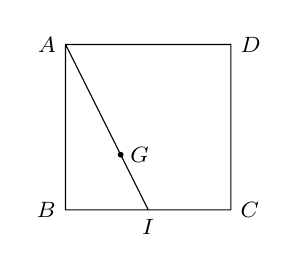
\begin{tikzpicture}[scale=0.7, font=\footnotesize, line join=round, line cap=round, >=stealth]
				\def\a{3} % độ dài cạnh hình vuông
				\draw (0,\a) node [left]{$A$}--(0,0) node [left]{$B$}--(\a,0) node [right]{$C$}--(\a,\a) node [right]{$D$}--(0,\a)--(\a/2,0) node [below]{$I$};
				\fill (\a/3,\a/3) circle (1.5pt) node [right]{$G$};
			\end{tikzpicture}
		}
	}
\end{ex}
\begin{ex}%[0H5H3-5]%[Dự án D - Đề cương 3 khối 10-11-12 NH25-26 - Nguyễn Tiến]%
	[\textit{Trích đề thi GHKI - Trường THPT Nguyễn Huệ, Thừa Thiên Huế - Năm học 2023-2024}]
	Cho tam giác $ABC$, $M$ là trung điểm của cạnh $BC$, điểm $N$ nằm trên cạnh $AC$ sao cho $NA=2NC$, $D$ là trung điểm của $AN$.
	\begin{enumerate}
		\item Chứng minh: $\overrightarrow{AC}+3 \overrightarrow{DA}=\overrightarrow{0}$.
		\item Phân tích véc-tơ $\overrightarrow{MN}$ theo hai véc-tơ $\overrightarrow{AB}$ và $\overrightarrow{AC}$.
	\end{enumerate}
	\loigiai{
		\immini{
			\begin{enumerate}
				\item Vì $NA=2NC$ và $D$ là trung điểm của $AN$ nên $AD=DN=NC=\dfrac{1}{3}AC$.\\
				Suy ra $\overrightarrow{AC}=-3\overrightarrow{DA}$.
				\item Ta có $\overrightarrow{MN}= \overrightarrow{AN}-\overrightarrow{AM}=\dfrac{2}{3}\overrightarrow{AC}-\dfrac{1}{2}\left(\overrightarrow{AB}+\overrightarrow{AC}\right)$.\\
				$\Rightarrow \overrightarrow{MN}=-\dfrac{1}{2}\overrightarrow{AB}+\dfrac{1}{6}\overrightarrow{AC}$.
			\end{enumerate}
		}{
			\begin{tikzpicture}[scale=0.6, font=\footnotesize, line join=round, line cap=round, >=stealth]
				\path
				(4,4) coordinate (A)
				(2,0) coordinate (B)
				(7,0) coordinate (C)
				($(B)!.5!(C)$) coordinate (M) ($(A)!2/3!(C)$) coordinate (N) ($(A)!1/3!(C)$) coordinate (D)
				;
				\draw (A)--(B)--(C)--cycle;
				\draw[->,thick,blue] (M)--(N);
				\path
				(A)--(B)--(C)--(A)
				;
				\foreach \p/\r in {A/90,B/-120,C/-60,M/-90,D/45,N/45}
				\fill (\p) circle (1.5pt) node[shift={(\r:3mm)}]{$\p$};
			\end{tikzpicture}
		}
	}
\end{ex}
\begin{ex}%[0H5V3-5]%[Dự án D - Đề cương 3 khối 10-11-12 NH25-26 - Nguyễn Tiến]%
	[\textit{Trích đề thi HKI - Trường THPT Nguyễn Văn Trỗi, Khánh Hoà - Năm học 2023-2024}]
	Cho tam giác $A B C$ và các điểm $P$, $Q$, $R$ được xác định như hình vẽ.
	\immini{
		\begin{enumerate}
			\item Biểu thị $\overrightarrow{P Q}$ và $\overrightarrow{P R}$ theo hai véc-tơ $\overrightarrow{A B}$ và $\overrightarrow{A C}$.
			\item Có thể nói gì về ba điểm $P$, $Q$ và $R$? Giải thích câu trả lời.
		\end{enumerate}
	}{
		\begin{tikzpicture}[scale=0.6, font=\footnotesize, line join=round, line cap=round, >=stealth]
			\path 
			(0,0) coordinate (B)
			(5,0) coordinate (C)
			($(B)!3/5!60:(C)$) coordinate (A)
			($(A)!1/3!(B)$) coordinate (P)
			($(A)!2/3!(B)$) coordinate (P')
			($(A)!1/4!(C)$) coordinate (Q1)
			($(A)!2/4!(C)$) coordinate (Q2)
			($(A)!3/4!(C)$) coordinate (Q)
			($(B)!1/5!(C)$) coordinate (M1)
			($(B)!2/5!(C)$) coordinate (M2)
			($(B)!3/5!(C)$) coordinate (M3)
			($(B)!4/5!(C)$) coordinate (M4)
			($(C)!1/5!180:(B)$) coordinate (R)
			;
			\draw (C)--(A)--(B)--(R);
			\foreach \x/\y in {A/90,B/190,C/-90,P/190,Q/40,R/-90}
			\draw[fill=black] (\x) circle (1.1pt) + (\y:0.5cm) node{$\x$};
			\foreach \x/\y in {P'/90,Q1/190,Q2/-90,M1/40,M2/-90,M3/90,M4/-90}
			\draw[fill=black] (\x) circle (1.1pt) + (\y:0.5cm) ;
		\end{tikzpicture}
	}
	\loigiai{
		\begin{enumerate}
			\item Ta có $\overrightarrow{P Q}=\overrightarrow{AQ}-\overrightarrow{A P}=\dfrac{3}{4}\overrightarrow{A C}-\dfrac{1}{3}\overrightarrow{A B}$.\\
			Lại có
			\allowdisplaybreaks
			\begin{eqnarray*}
				\overrightarrow{P R} &= & \overrightarrow{PB}+\overrightarrow{BR}=\dfrac{2}{3}\overrightarrow{AB}+\dfrac{6}{5}\overrightarrow{BC}\\
				&= & \dfrac{2}{3}\overrightarrow{ AB}+\dfrac{6}{5}\cdot \left(\overrightarrow{AC}-\overrightarrow{AB}\right)\\
				&= & \dfrac{6}{5}\overrightarrow{AC}-\dfrac{8}{15}\overrightarrow{AB}.
			\end{eqnarray*}
			\item $\overrightarrow{PQ}=\dfrac{5}{8}\overrightarrow{PR}$. Do đó $P$, $Q$, $R$ thẳng hàng.
		\end{enumerate}
	}
\end{ex}
\begin{ex}%[0H5V3-4]%[Dự án D - Đề cương 3 khối 10-11-12 NH25-26 - Nguyễn Tiến]%
	[\textit{Trích đề thi HKI - Trường THPT Phan Bội Châu, Bình Thuận - Năm học 2023-2024}]
	Cho tam giác $ABC$ có $M$ là trung điểm $BC$. Gọi $I$, $K$ là hai điểm thỏa $\overrightarrow{AI}=\dfrac{1}{3}\overrightarrow{AM}$, $\overrightarrow{AK}=\dfrac{1}{5}\overrightarrow{AC}$. Chứng minh ba điểm $B$, $I$, $K$ thẳng hàng.
	\loigiai{
		\immini{
			Ta có
			\allowdisplaybreaks
			\begin{eqnarray*}
				\overrightarrow{BI}&=&\overrightarrow{BA}+\overrightarrow{A I} =-\overrightarrow{AB}+\dfrac{1}{3} \overrightarrow{A M}\\
				&=&-\overrightarrow{A B}+\dfrac{1}{3} \cdot \dfrac{1}{2}(\overrightarrow{A B}+\overrightarrow{A C})\\
				&=&-\dfrac{5}{6} \overrightarrow{A B}+\dfrac{1}{6} \overrightarrow{A C}.
			\end{eqnarray*}
			$\Rightarrow 6\overrightarrow{B I}=-5 \overrightarrow{A B}+\overrightarrow{A C}. \hfill(1)$\\
			Mặt khác $ \overrightarrow{B K}=\overrightarrow{A K}-\overrightarrow{A B}
			=\dfrac{1}{5} \overrightarrow{A C}-\overrightarrow{A B}$.\\
			$\Rightarrow 5\overrightarrow{B K}=\overrightarrow{A C}-5 \overrightarrow{A B}.\hfill (2)$\\
			Từ $(1)$ và $(2)$ suy ra $6 \overrightarrow{B I}=5 \overrightarrow{B K} \Leftrightarrow \overrightarrow{B I}=\dfrac{5}{6} \overrightarrow{B K}$.\\
			Vậy ba điểm $B$, $I$, $K$ thẳng hàng.
		}{
			\begin{tikzpicture}[scale=1, font=\footnotesize, line join=round, line cap=round, >=stealth]
				\coordinate (B) at (0,0);
				\coordinate (C) at (3,0); \coordinate (A) at (1,2.5);
				\coordinate (M) at ($(B)!0.5!(C)$);
				\coordinate (I) at ($(A)!0.33!(M)$);
				\coordinate (K) at ($(A)!0.2!(C)$);
				\pgfresetboundingbox %Co khung hình 
				\draw (A)--(B)--(C)--cycle (I)--(B)--(K)  (A)--(M);
				\foreach \x/ \goc in {A/135,B/-135,C/-45,I/135,K/0,M/-45} 
				\fill (\x) circle (1pt)
				($(\x)+(\goc:3mm)$) node {$\x$};	   
			\end{tikzpicture}
		}
	}
\end{ex}
\begin{ex}%[0H5V3-5]%[Dự án D - Đề cương 3 khối 10-11-12 NH25-26 - Nguyễn Tiến]%
	[\textit{Trích đề thi HKI - Trường THPT Phạm Văn Sáng, TPHCM - Năm học 2023-2024}]
	Cho tam giác $ABC$. Trên cạnh $AC$ lấy điểm $I$ sao cho $AI=2IC$. Chứng minh rằng $\overrightarrow{BA}+2\overrightarrow{BC}=3\overrightarrow{BI}$.
	\loigiai{
		\immini{
			Ta có
			\allowdisplaybreaks
			\begin{eqnarray*}
				\overrightarrow{BI} &= & \overrightarrow{AI}-\overrightarrow{AB}=\dfrac{2}{3}\overrightarrow{AC}-\overrightarrow{AB} \\
				&= & \dfrac{2}{3}\left(\overrightarrow{BC}-\overrightarrow{BA}\right)+\overrightarrow{BA} \\
				&= & \dfrac{2}{3}\overrightarrow{BC}+\dfrac{1}{3}\overrightarrow{BA}.
			\end{eqnarray*}
		}{
			\begin{tikzpicture}[scale=0.7, font=\footnotesize, line join=round, line cap=round, >=stealth]
				\path (0,0) coordinate (B) (1,3) coordinate (A) (4,0) coordinate (C)
				($(A)!2/3!(C)$) coordinate (I)
				;
				\draw (A)--(B)--(C)--cycle (B)--(I);		
				\foreach \x/\g in {A/90,B/180,C/0,I/45}
				\fill[black] 	(\x) circle (1pt)
				($(\g:3mm)+(\x)$) node {$\x$};
			\end{tikzpicture}
		}
		Vậy $3\overrightarrow{BI} = \overrightarrow{BA}+2\overrightarrow{BC}$.
	}
\end{ex}
\begin{ex}%[0H5V3-8]%[Dự án D - Đề cương 3 khối 10-11-12 NH25-26 - Nguyễn Tiến]%
	[\textit{Trích đề thi HKI - Sở Giáo dục và Đào tạo Bắc Ninh - Năm học 2023-2024}]
	Cho tam giác $ABC$ vuông tại $A$, có $AB=3, BC=5$. Gọi $E$ là trung điểm $AB$.
	\begin{enumerate}
		\item Chứng minh $2\overrightarrow{AE}+\overrightarrow{CA}=\overrightarrow{CB}$.
		\item Xác định điểm $I$ thỏa mãn $\overrightarrow{IA}+\overrightarrow{IB}+2\overrightarrow{IC}=\overrightarrow0$.
		\item Gọi $M$ là điểm thay đổi trên đường thẳng $BC$. Tìm giá trị nhỏ nhất của biểu thức
		\[T=\left|\overrightarrow{MA}+\overrightarrow{MB}+2\overrightarrow{MC}\right|.\]
	\end{enumerate}
	\loigiai{
		\immini{
			\begin{enumerate}
				\item Vì $E$ là trung điểm $AB$ nên $\overrightarrow{AB}=2\overrightarrow{AE}$.\\
				Suy ra $VT=2\overrightarrow{AE}+\overrightarrow{CA}=\overrightarrow{AB}+\overrightarrow{CA}=\overrightarrow{CB}=VP$ (đpcm).
				\item Ta có
				\allowdisplaybreaks
				\begin{eqnarray*}
					& & \overrightarrow{IA}+\overrightarrow{IB}+2\overrightarrow{IC}=\overrightarrow 0\\
					&\Leftrightarrow & 2\overrightarrow{IE}+2\overrightarrow{IC}=\overrightarrow 0\\
					&\Leftrightarrow & \overrightarrow{IE}+\overrightarrow{IC}=\overrightarrow 0.
				\end{eqnarray*}
				Suy ra $I$ là trung điểm của $EC$.
			\end{enumerate}
		}{
			\begin{tikzpicture}[scale=0.7, font=\footnotesize, line join=round, line cap=round, >=stealth]
				\path 
				(0:0) coordinate (A)++(0:4) coordinate (C)
				(A)++(90:3) coordinate (B)
				($(B)!1/2!(A)$) coordinate (E)
				($(E)!1/2!(C)$) coordinate (I)
				($(B)!9/25!(C)$) coordinate (H)
				($(B)!1/2!(H)$) coordinate (J)
				($(J)!1/2!(C)$) coordinate (K)
				;
				\draw 
				(A)--(B)--(C)--(A) (C)--(E) (E)--(J) (A)--(H) (I)--(K)
				;
				\pic[draw,thin,angle radius=2mm] {right angle = E--J--B}
				pic[draw,thin,angle radius=2mm] {right angle = A--H--B}
				pic[draw,thin,angle radius=2mm] {right angle = I--K--B}
				;
				\foreach \x/\g in {E/180,B/100,A/-150,C/-20,I/-120,J/60, H/60, K/60}
				\fill (\x) circle (1pt)
				+(\g:3mm) node{$\x$};
			\end{tikzpicture}
		}
		\noindent
		\begin{enumerate}
			\setcounter{enumi}{2}
			\item Ta có
			\begin{eqnarray*}
				T & = & \left|\overrightarrow{MI}+\overrightarrow{IA}+\overrightarrow{MI}+\overrightarrow{IB}+2\left(\overrightarrow{MI}+\overrightarrow{IC}\right)\right| \\
				& = & \left|4\overrightarrow{MI}+\overrightarrow{IA}+\overrightarrow{IB}+2\overrightarrow{IC}\right|\\
				& = & \left|4\overrightarrow{MI}+\overrightarrow{0}\right|=\left|4\overrightarrow{MI}\right|=4MI.			
			\end{eqnarray*}
			Tam giác $ABC$ vuông tại $A$ nên $AC=\sqrt{BC^2 - AB^2} = 4$.\\
			Do $M$ di động trên đường thẳng $BC$, nên $T$ đạt giá trị nhỏ nhất khi $M\equiv K$, với $K$ là hình chiếu của $I$ trên đường thẳng $BC$.\\	
			Gọi $J$, $H$ lần lượt là hình chiếu vuông góc của $E$ và $A$ xuống cạnh $BC$.\\
			Suy ra $IK$, $AH$, $EJ$ đôi một song song với nhau.\\
			Dễ thấy $IK=\dfrac{1}{2} EJ=\dfrac{1}{4} AH$.\\	
			Vậy $\min T=4IK=AH=\dfrac{AB\cdot AC}{BC}=\dfrac{3\cdot 4}{5}=\dfrac{12}{5}$.
		\end{enumerate}
	}
\end{ex}